% Options for packages loaded elsewhere
\PassOptionsToPackage{unicode}{hyperref}
\PassOptionsToPackage{hyphens}{url}
\documentclass[
]{book}
\usepackage{xcolor}
\usepackage{amsmath,amssymb}
\setcounter{secnumdepth}{5}
\usepackage{iftex}
\ifPDFTeX
  \usepackage[T1]{fontenc}
  \usepackage[utf8]{inputenc}
  \usepackage{textcomp} % provide euro and other symbols
\else % if luatex or xetex
  \usepackage{unicode-math} % this also loads fontspec
  \defaultfontfeatures{Scale=MatchLowercase}
  \defaultfontfeatures[\rmfamily]{Ligatures=TeX,Scale=1}
\fi
\usepackage{lmodern}
\ifPDFTeX\else
  % xetex/luatex font selection
\fi
% Use upquote if available, for straight quotes in verbatim environments
\IfFileExists{upquote.sty}{\usepackage{upquote}}{}
\IfFileExists{microtype.sty}{% use microtype if available
  \usepackage[]{microtype}
  \UseMicrotypeSet[protrusion]{basicmath} % disable protrusion for tt fonts
}{}
\makeatletter
\@ifundefined{KOMAClassName}{% if non-KOMA class
  \IfFileExists{parskip.sty}{%
    \usepackage{parskip}
  }{% else
    \setlength{\parindent}{0pt}
    \setlength{\parskip}{6pt plus 2pt minus 1pt}}
}{% if KOMA class
  \KOMAoptions{parskip=half}}
\makeatother
\usepackage{longtable,booktabs,array}
\newcounter{none} % for unnumbered tables
\usepackage{calc} % for calculating minipage widths
% Correct order of tables after \paragraph or \subparagraph
\usepackage{etoolbox}
\makeatletter
\patchcmd\longtable{\par}{\if@noskipsec\mbox{}\fi\par}{}{}
\makeatother
% Allow footnotes in longtable head/foot
\IfFileExists{footnotehyper.sty}{\usepackage{footnotehyper}}{\usepackage{footnote}}
\makesavenoteenv{longtable}
\usepackage{graphicx}
\makeatletter
\newsavebox\pandoc@box
\newcommand*\pandocbounded[1]{% scales image to fit in text height/width
  \sbox\pandoc@box{#1}%
  \Gscale@div\@tempa{\textheight}{\dimexpr\ht\pandoc@box+\dp\pandoc@box\relax}%
  \Gscale@div\@tempb{\linewidth}{\wd\pandoc@box}%
  \ifdim\@tempb\p@<\@tempa\p@\let\@tempa\@tempb\fi% select the smaller of both
  \ifdim\@tempa\p@<\p@\scalebox{\@tempa}{\usebox\pandoc@box}%
  \else\usebox{\pandoc@box}%
  \fi%
}
% Set default figure placement to htbp
\def\fps@figure{htbp}
\makeatother
% definitions for citeproc citations
\NewDocumentCommand\citeproctext{}{}
\NewDocumentCommand\citeproc{mm}{%
  \begingroup\def\citeproctext{#2}\cite{#1}\endgroup}
\makeatletter
 % allow citations to break across lines
 \let\@cite@ofmt\@firstofone
 % avoid brackets around text for \cite:
 \def\@biblabel#1{}
 \def\@cite#1#2{{#1\if@tempswa , #2\fi}}
\makeatother
\newlength{\cslhangindent}
\setlength{\cslhangindent}{1.5em}
\newlength{\csllabelwidth}
\setlength{\csllabelwidth}{3em}
\newenvironment{CSLReferences}[2] % #1 hanging-indent, #2 entry-spacing
 {\begin{list}{}{%
  \setlength{\itemindent}{0pt}
  \setlength{\leftmargin}{0pt}
  \setlength{\parsep}{0pt}
  % turn on hanging indent if param 1 is 1
  \ifodd #1
   \setlength{\leftmargin}{\cslhangindent}
   \setlength{\itemindent}{-1\cslhangindent}
  \fi
  % set entry spacing
  \setlength{\itemsep}{#2\baselineskip}}}
 {\end{list}}
\usepackage{calc}
\newcommand{\CSLBlock}[1]{\hfill\break\parbox[t]{\linewidth}{\strut\ignorespaces#1\strut}}
\newcommand{\CSLLeftMargin}[1]{\parbox[t]{\csllabelwidth}{\strut#1\strut}}
\newcommand{\CSLRightInline}[1]{\parbox[t]{\linewidth - \csllabelwidth}{\strut#1\strut}}
\newcommand{\CSLIndent}[1]{\hspace{\cslhangindent}#1}
\setlength{\emergencystretch}{3em} % prevent overfull lines
\providecommand{\tightlist}{%
  \setlength{\itemsep}{0pt}\setlength{\parskip}{0pt}}
\usepackage[spanish,es-tabla]{babel}
\usepackage{bookmark}
\IfFileExists{xurl.sty}{\usepackage{xurl}}{} % add URL line breaks if available
\urlstyle{same}
\hypersetup{
  pdftitle={Estadística Aplicada},
  pdfauthor={Equipo Editorial, Wulfrano Gómez Gallardo},
  hidelinks,
  pdfcreator={LaTeX via pandoc}}

\title{Estadística Aplicada}
\author{Equipo Editorial, Wulfrano Gómez Gallardo}
\date{2026-09-23}

\begin{document}
\maketitle

{
\setcounter{tocdepth}{2}
\tableofcontents
}
\chapter{MUESTRA Y PROBLACIÓN}\label{muestra-y-problaciuxf3n}

\section{POBLACIÓN}\label{poblaciuxf3n}

Una población, en estadística, es un conjunto de elementos que comparten una característica en común de interés para un investigador.

Como ejemplos podemos mencionar el interés de un investigador sobre el uso de celulares entre estudiantes de secundaria en México. En este caso la población está integrada por todos los mexicanos que se encuentren actualmente inscritos en una institución educativa, pública o privada a nivel secundaria. También podría ser del interés de un investigador ciertas especies y su capacidad de reproducción. Por ejemplo, las plagas que afectan las grandes ciudades como son las ratas. En este caso se podría establecer la cantidad de roedores que se concentran en una ciudad, para establecer como se reproducen o migran a estas grandes ciudades como Nueva York.

Las poblaciones pueden ser finitas o infinitas, de ellas se pueden medir características cuantitativas o cualitativas. Como ejemplo de poblaciones infinitas podemos mencionar el lanzamiento de una moneda un número infinito de veces, los números que se encuentran entre cero y uno, que poden ser seleccionados al azar, entre otros. Mientras que las poblaciones finitas pueden estar representadas por ciudadanos en un país, número de especies en una región, entre otros. Las características cuantitativas que se pueden medir de estas poblaciones pueden ser edad, estaturas, pesos, entre otros. Mientras que las características cuantitativas como color de ojos, color de la piel, entre otros.

Las características cualitativas siempre deben ser cuantificadas de forma cuantitativa para fines estadísticos, a estas variables se les conoce como factores. Por ejemplo el nivel de satisfacción de por u servicio recibido, los cuales son representados por figuras para hacer que el usuario pueda responde de la forma más objetiva y de manera sencilla, como se muestra en la figura 1\footnote{\emph{Fuente: Extraido de \url{https://www.magnific.com/es/vector-gratis/medidor-satisfaccion-emoji-pequeno_44156211.htm\#fromView=keyword&page=1&position=0&uuid=484b5e55-bf2d-4120-b59f-55c1c2d67403&track=ais_hybrid&query=Caritas+satisfaccion}}}

\begin{figure}
\centering
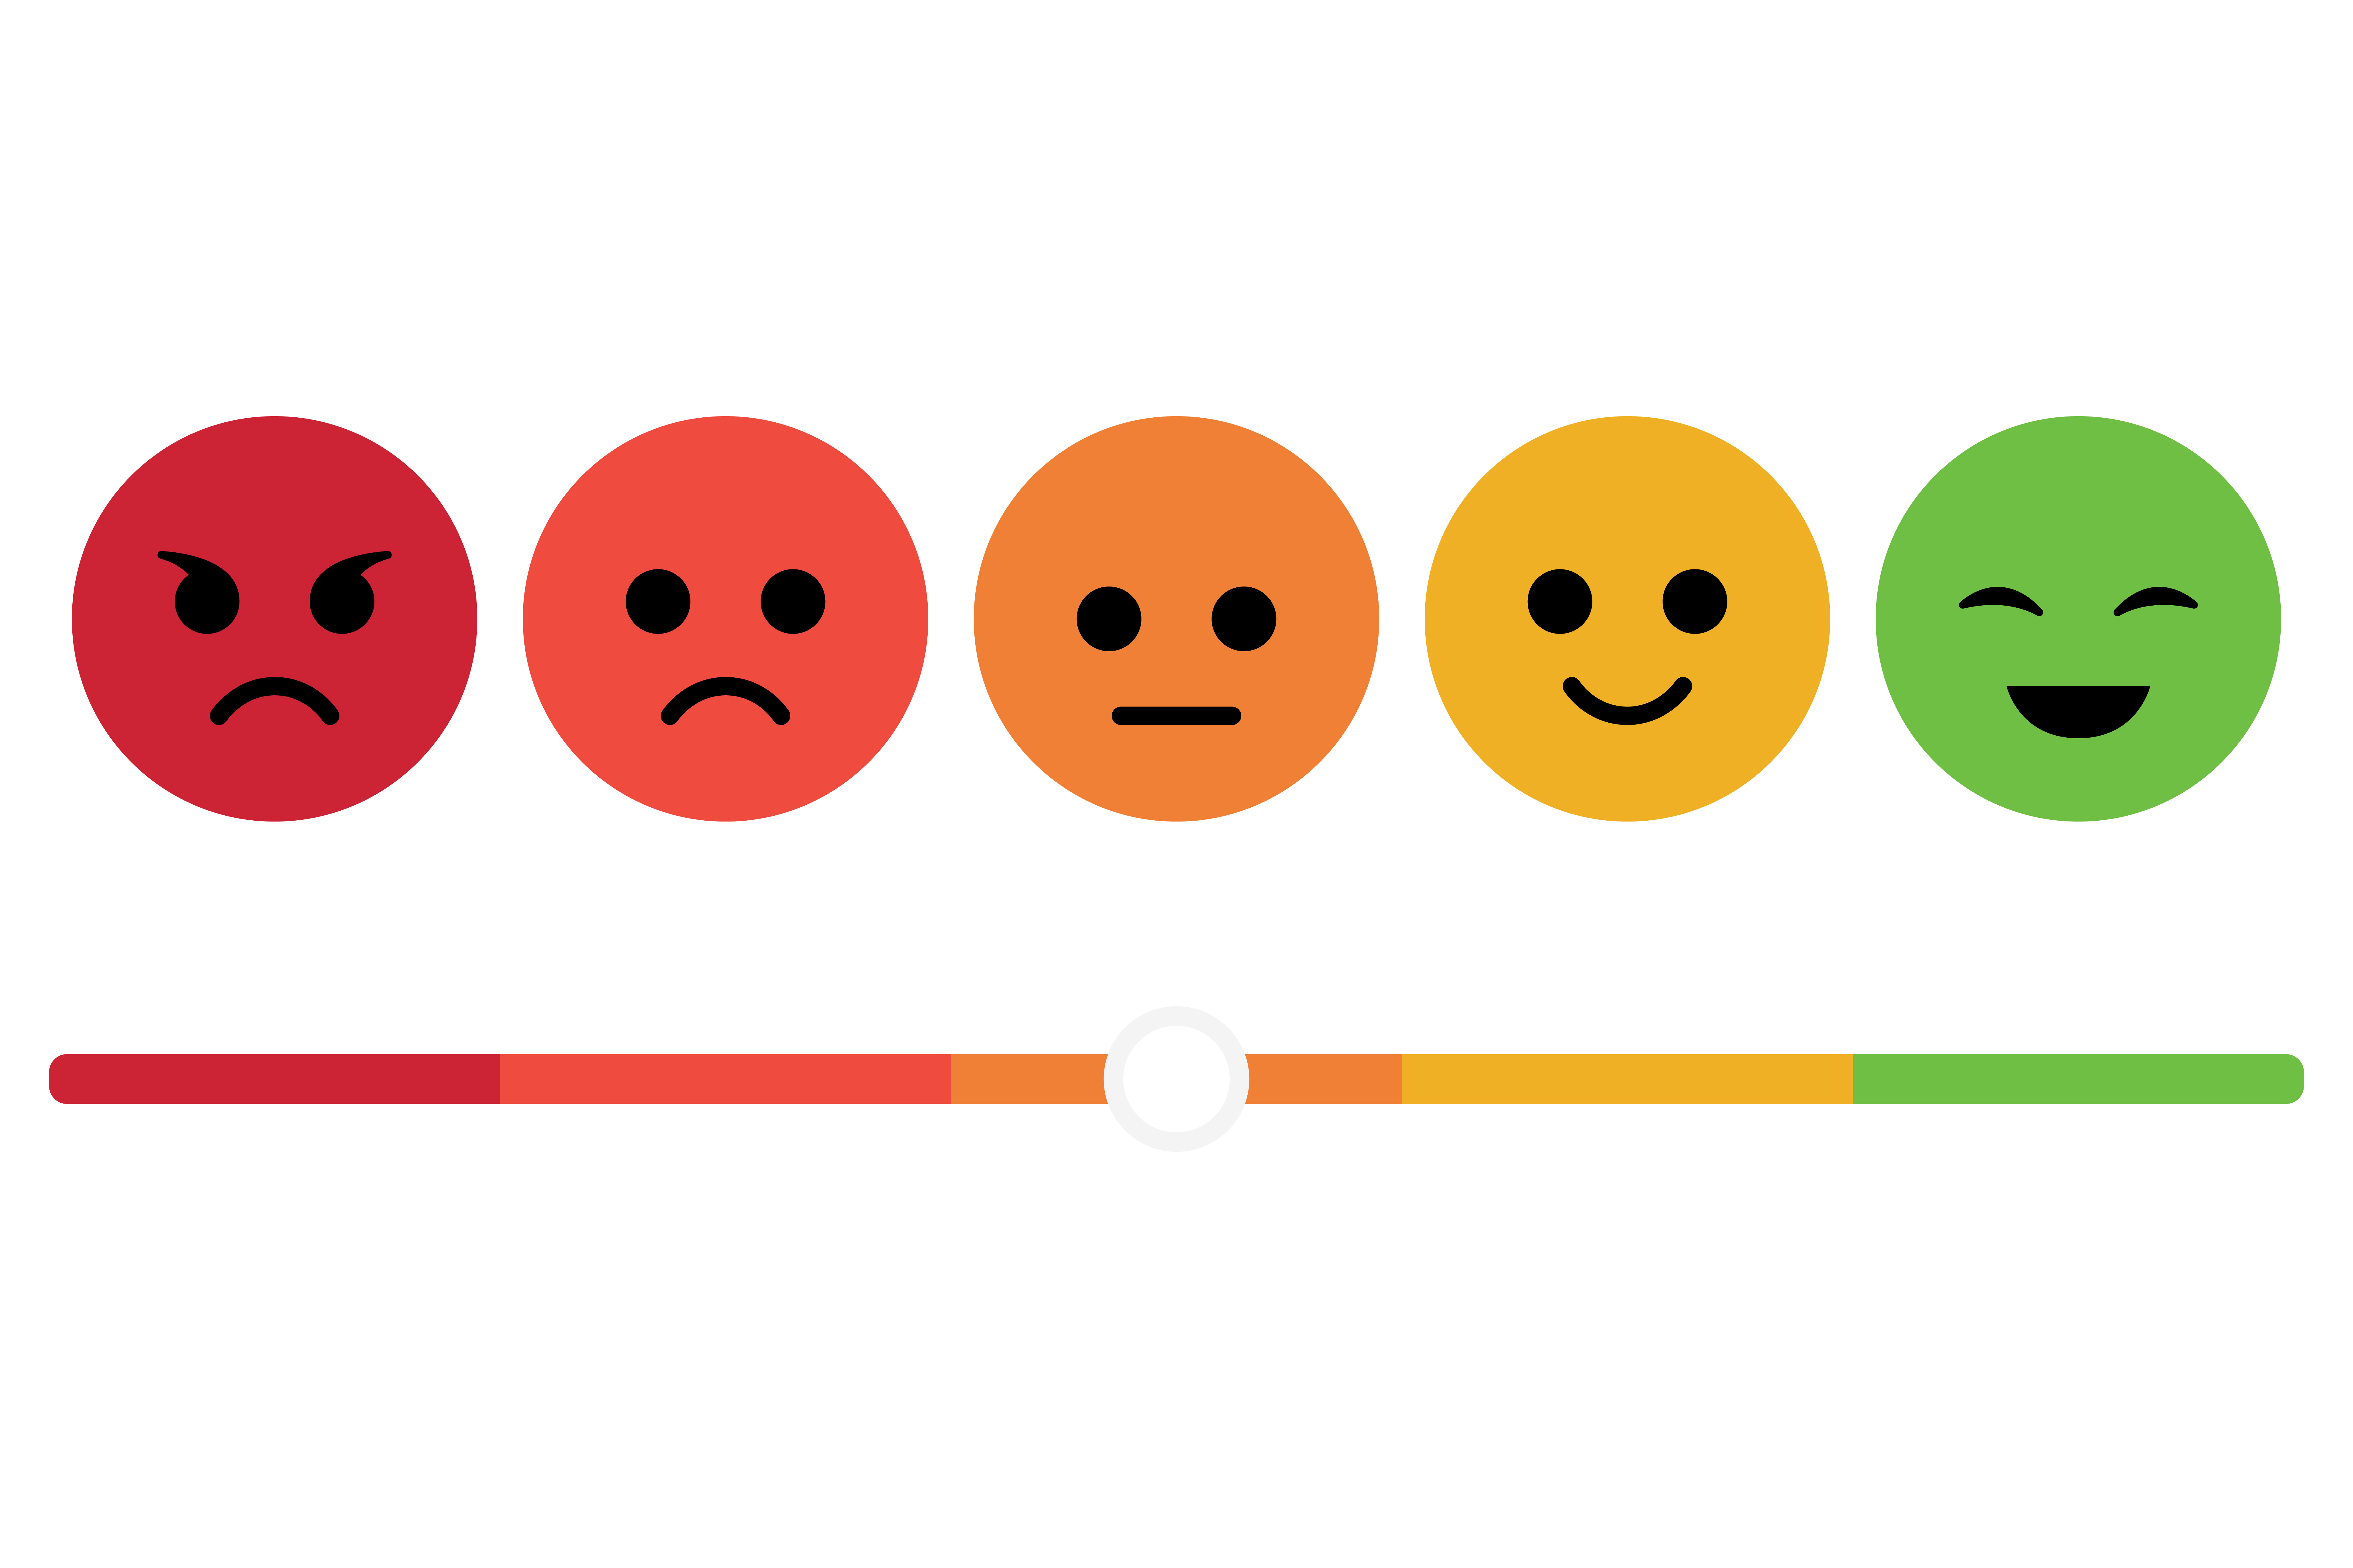
\includegraphics[width=0.4\linewidth,height=\textheight,keepaspectratio,alt={Encuesta de satisfacción}]{images/emoji_satisfaction_meter.jpg}
\caption{Encuesta de satisfacción}\label{fig:satisfaccion}
\end{figure}

Debido a que las poblaciones pueden ser demasiado grandes para censarlas o el tiempo es limitado para realizar el censo, o no se cuentan con los recursos económicos necesarios, es que se deben realizar muestreos.

\section{Muestreo}\label{muestreo}

Una muestra es un subconjunto de la población que se selecciona de forma aleatoria, representativa e insesgada.

¿Qué significa esto?

\begin{itemize}
\tightlist
\item
  Aleatorio: Los elementos se seleccionan sin un orden específico. Esto es, no se sabe qué elemento será seleccionado. Generalmente se generan números aleatorios o se seleccionan los elementos de una tómbola.
\item
  Representativo: En este caso se espera que los elementos de la población queden representados en la muestra. suponga que una población de 1,000 personas, con un 20\% de mujeres y un 80\% de hombres, la muestra debería tener al menos un número suficientes de representates de hombres y mujeres. Por ejemplo, si una muestra de 100 elementos de esta población que se toma de manera aleatoria, podría conducir a que todos los elementos seleccionados fueran hombres y ninguna mujer, esta muestra no sería representativa.
\item
  Insesgado: Se espera que la muestra sea aleatoria, lo que evitaría algún criterio de selección e los elementos de la muestra por parte del investigador. Por ejemplo: Suponga que una acreditadora desea seleccionar a diez estudiantes de manera aleatoria de un grupo de matemáticas, para aplicarles una prueba y evaluar el desempeño del profesor. Suponga también que el profesor será recompensado si los estudiantes seleccionados aleatoriamente obtiene buenos resultados, en caso contrario, su contrato será rescindido. El profesor podría verse tentado a seleccionar solo a los alumnos con mejor promedio para este fin, lo que provocaría un sesgo al seleccionar dicha muestra.
\end{itemize}

\section{ESTIMADORES}\label{estimadores}

Debido a que las poblaciones son demasiado grandes para censarlas o el tiempo para realizar el censo es limitado, así como los recursos financieros y humanos, es que nos vemos en la necesidad de realizar muestreo. Es necesario realizar estimaciones de los parámetros poblacionales que deseamos conocer. Esto es, si el objetivo fuera calcular la estatura promedio de los estudiantes de la facultad de ingeniería y sólo tuviéramos un par de días para hacerlo, a través de una muestra se estiman los parámetros poblacionales, en este caso la media. Entonces se dice que la media muestral \(\bar{x}\) estima al parámetro poblacional \(\mu\).

La diferencia en el cálculo de la media de una muestra y de una poblacional es la siguiente

\textbf{Media muestral}

\begin{equation}
\bar{x}=\frac{1}{n}\sum_{i=1}^{n}x_i
\end{equation}

en donde

\(\boldsymbol{\bar{x}}\) : Es la media muestral.

\(\boldsymbol{n}\): es el tamaño de la muestra y representa la probabilidad de seleccionar un elemento. En este caso todos los elementos de la muestra son equiprobables. Esto es, tiene la misma probabilidad de ser seleccionados.

\(\boldsymbol{x_i}\): es el elemento i-ésimo, seleccionado de la población de forma aleatoria.

\textbf{Media poblacional}

En el caso de una variable aleatoria\footnote{Una variable aleatoria para este fin se considera un evento asociado a una probabilidad} discreta

\begin{equation}
\mu=\sum_{i=1}^Nx_ip(x_i)
\end{equation}

en donde:

\(\boldsymbol{\mu}\): es la media poblacional.

\(\boldsymbol{N}\): es el tamaño de la población.

\(\boldsymbol{p(x_i)}\): es la medida de la probabilidad del evento \(\boldsymbol{x_i}\).

\(\boldsymbol{x_i}\): es el i-esimo elemento de la población.

En este caso se dice que el estadístico \(\bar{x}\) estima al parámetro \(\mu\). Esto es

\(\bar{X}\) estima a \(\mu\)

{\emph{\textbf{La siguiente aplicación ejemplifica esto}}}

Es claro que el valor del estadístico no corresponderá exactamente al valor del parámetro, debido a que el primero se calcula con un subconjunto de de los elementos de la población.

¿Por qué entonces podemos confiar en un estadístico de una muestra para estimar un parámetro poblacional?

\chapter{DISTRIBUCIONES MUESTRALES}\label{distribuciones-muestrales}

Una distribución de muestras, es el resultado de tomar la combinación de un tamaño \textbf{\emph{n}} de elementos de una población de tamaño \textbf{\emph{N}} generando \textbf{\emph{K}} combinaciones y calculando \(\boldsymbol{\bar{x}_k}\) medias muestrales, las cuales resultan ser variables aleatorias (v.a.). Esto es, si se seleccionan diferentes muestras, del mismo tamaño n de forma aleatoria, de una población, cada una de ellas tendría un valor diferente y la probabilidad de que alguna de ellas acierte al valor del parámetro poblacional \(\boldsymbol{\mu}\) es casi seguramente cero.

En forma matemática se tiene

\begin{equation}
C(N,n)=\binom{N}{n}=\frac{N!}{n!(N-n)!}=K
\label{eq:combinaciones}
\end{equation}

en donde

\(K\): es el número de combinaciones de tamaño \(n\) tomadas de \(N\).

En este caso la varianza de las medias de las muestras se calcula como

\begin{equation}
\sigma^2_{\bar{x}}=\frac{\sum_{i=1}^K(\bar{X}_i-\bar{\bar{X}})^2}{k}
\label{eq:varianza_muestral}
\end{equation}

donde

\begin{equation}
\bar{\bar{X}}=\frac{\sum_{i=1}^k\bar{X}_i}{K}
\label{eq:media_medias}
\end{equation}

\(\bar{\bar{X}}\): media de las medias.

y la i-ésima media de las muestras, con un tamaño demuestra \textbf{n} es

\begin{equation}
\bar{X}_i=\frac{\sum_{j=1}^nX_j}{n}
\label{eq:media_mues}
\end{equation}

En este caso el error estándar se obtiene al sacar la raíz cuadrada de la ecuación \eqref{eq:varianza_muestral}

\begin{equation}
\sigma_{\bar{x}}=\sqrt{\sigma^2_{\bar{x}}}
\label{eq:err_est}
\end{equation}

Como se puede observar, el cálculo del error estándar por este procedimiento no es recomendable ya que existen más combinaciones \textbf{\emph{K}} que el número de elementos de la población \textbf{\emph{N}}. lo que lo hace poco práctico o inservible si se desea calcular. Esto es, es más fácil censar a la población, que tomar todas las combinaciones de las muestras de tamaño \textbf{\emph{n}} para calcular el error estándar.

En este caso, considere las variables aleatorias

\begin{equation}
X_1,X_2,...,X_n
\label{eq:va}
\end{equation}

En donde

\begin{equation}
E[X_i]=\mu
\label{eq:esp}
\end{equation}

y su varianza es

\begin{equation}
Var[X_i]=\sigma^2
\label{eq:var}
\end{equation}

De la ecuación \eqref{eq:media_mues}, la media muestral es

\begin{equation}
\bar{X}=\frac{X_1+X_2+\dots+X_n}{n}
\label{eq:media_va}
\end{equation}

y su varianza

\begin{equation}
Var[\bar{X}]=Var\left[\frac{X_1+X_2+\dots+X_n}{n}\right]
\label{eq:var_mues}
\end{equation}

en donde

\begin{equation}
Var[\bar{X}]=\frac{Var[X_1]+Var[X_2]+\dots+Var[X_n]}{n^2}
\label{eq:var_mues2}
\end{equation}

de la ecuación \eqref{eq:var_mues} se tiene

\begin{equation}
Var[\bar{X}]=\frac{n\sigma^2}{n^2}
\end{equation}

donde

\begin{equation}
Var[\bar{X}]=\frac{\sigma^2}{n}
\end{equation}

y finalmente el error estándar es

\begin{equation}
\sigma_{\bar{x}}=\sqrt{\frac{\sigma^2}{n}}=\frac{\sigma}{\sqrt{n}}
\end{equation}

\section{Teorema del Límite Central}\label{teorema-del-luxedmite-central}

Sean \(X_1,X_2,...,X_n\) una muestra de tamaño \textbf{n} de una población de tamaño \textbf{N} con media \(\mu\) y varianza finita \(\sigma^2\), de esta población se obtienen \textbf{k} combinaciones de tamaño \textbf{n}, que generan \(\bar{X}_k\) medias muestrales, estas últimas tienden a distribuirse de forma asintótica a la normal con media \(\bar{\bar{X}}=\mu\) y error estándar \(\sigma_{\bar{x}}\), el cual disminuye conforme el tamaño de la muestra aumenta, no importando la distribución de probabilidad de la que provengan las variables aleatorias de las muestras tomadas.

La figura 2 ejemplifica esto.

\begin{figure}
\centering
\pandocbounded{
\includegraphics[keepaspectratio,alt={\label{fig:TLC}Teorema del Límite Central}]{bookdownproj_files/figure-latex/TLC-1.pdf}}
\caption{\label{fig:TLC}Teorema del Límite Central}
\end{figure}

\section{ESTIMACIÓN PUNTUAL}\label{estimaciuxf3n-puntual}

Como se puede observar los valores de \(\bar{X}_i\) se distribuyen de forma gaussiana alrededor de \(\bar{\bar{X}}=\mu\) y a medida que el tamaño de la muestra aumenta, el error estándar disminuye y los valores se encuentran más cerca del parámetro poblacional \(\mu\). Sin embargo, la probabilidad de que alguna \(\bar{X}_i\) sea igual al parámetro desconocido \(\mu\) es casi seguramente de cero, aún si el valor fuera igual o casi igual al parámetro no lo sabría, por eso la estimación puntual del parámetro no es recomendable, por lo que es necesario utilizar un intervalo donde se pueda establecer, con un error específico y una probailidad, que se encontrará el parámetro real pero desconocido.

\chapter{INTERVALOS DE CONFIANZA}\label{intervalos-de-confianza}

Un intervalo de confianza se establece como la probabilidad de que el parámetro desconocido \(\mu\) se encuentre en un rango de valores, a dicha probabilidad asociada se le conoce como \textbf{coeficiente de confianza} \(cc=1-\alpha\) y se calcula al restar a uno el nivel de significancia \(\alpha\). Tanto el coeficiente de confianza como el nivel de significancia tienen un rango de valores aceptados. Por ejemplo, el \emph{cc} se acepta se encuentre \(90\%\leq cc<100\%\), mientras que \(0\%<\alpha\leq10\%\).

En este caso, si a la media poblacional se le colocan un par de brazos, uno a la izquierda y el otro a la derecha, con tamaño \(2\sigma_{\bar{x}}\) se tendrían el 95.5\% de las \(\bar{x}_i\) y solo el 4.5\% no los contendría. Sin embargo, como no se conoce el valor de \(\mu\) se deben colocar estos brazos en lo que sí se conoce \(\bar{X}_i\) y suponer que existe un 95.5\% de probabilidad de que este contenga a la media poblacional.

La razón por la que se usa la variable aleatoria \(z_i\), que corresponde a una variable aleatoria con distribución gaussina, específicamente la normal estándar con media \(\mu_z=0\) y desviación estándar \(\sigma_z=1\), es por que las distribuciones muestrales, como se ha establecido en el Teorema del Límite Central, se distribuyen de forma normal.

El tamaño del brazo que se le coloca a la media muestral se le conoce como error y se calcula con

\begin{equation}
E=z_{\frac{\alpha}{2}}\frac{\sigma}{\sqrt{n}}
\end{equation}

En donde

\(E\): Error de muestreo

\(z_{\frac{\alpha}{2}}\): Es el valor de la distribución \textbf{\emph{z}} que nos indica el número de desviaciones estándar a la izquierda y a la derecha en el que se concentran el 95.5\% de los elementos en una distribución normal estándar.

\(\sigma\): Es la desviación estándar poblacional.

\(n\): Es el tamaño de la muestra.

En este caso se suma y se resta este error \textbf{\emph{E}} a la \(\bar{X}_i\) para obtener los límites de confianza inferior y superiro.

\begin{equation}
IC=\bar{X}_i\pm E.
\end{equation}

En done

\(IC\): Intervalo de confianza

\(E\): Error de mustreo

Esto es

\begin{equation}
LI=\bar{X}_i-z_{\frac{\alpha}{2}}\frac{\sigma}{\sqrt{n}}
\end{equation}

y

\begin{equation}
LS=\bar{X}_i+z_{\frac{\alpha}{2}}\frac{\sigma}{\sqrt{n}}
\end{equation}

En donde

\(LS\): Límite superiro.

\(LI\): Límite inferior.

La siguiente aplicación ejemplifica el uso de dichos intervalos

\textbf{\emph{COLOCAR LIGA DE APP}}

Un ejemplo del uso de los intervalos de confianza se presenta a continuación.

\textbf{Ejemplo 1:}

Suponga que se desea estimar la estatura promedio de los estudiantes de la Facultad de Ingeniería, se sabe que la desviación estándar poblacional es de 9 cm. Una muestra de 31 alumnos reporta la siguiente media muestral \(\bar{x}\) = 167 cm. Suponga que se desea estimar a la media poblacional con una probabilidad del 95.5\%.

\textbf{Solución}

En este caso, el error de muestreo es de \(E\)= \(\pm\) 3.24 cm. El límite inferior \(LI\)= 63.76 y el límite superior \(LS\)= 70.24. Lo que significa que existe un 95.5\% de probabilidad de que la media poblacional de la estatura se encuentre entre estos valores. Es obvio que si se aumenta el tamaño de la muestra se incrementa el Error disminuye. Esto se verá en el ejemplo 2.

\textbf{Ejemplo 2:}

Suponga que en el ejemplo 1, el tamaño de la muestra es de 60 elementos. ¿Cuál sería el error de muestreo \textbf{\emph{E}}?

\textbf{Solución}

El nuevo error de muestreo con una muestra de 62 es de \(E\)= \(\pm\) 2.29 cm, el cual es menor al error \(E\)= \(\pm\) 3.24 cm con una muestra de 31 estudiantes. Como puede observarse, a pesar de que el tamaño de la muestra se duplicó, el error de muestreo no se redujo a la mitad.

Este tema será profundizado con mayor detalle en el siguiente capítulo, en donde se abordarán temas relacionados con el muestreo aleatorio irrestricto. También se analizará la situación cuando \(\sigma\) no sea conocida y qué pasa cuando la población que se analiza, el interés del investigador se centre en las proporciones.

En otras ocasiones el interés del investigador es el de encontrar el valor del parámetro que describe a una población, o la probabilidad de que este sea mayor o menor que un valor predeterminado, para esto se emplea una prueba de hipótesis.

\chapter{PRUEBAS DE HIPÓTESIS}\label{pruebas-de-hipuxf3tesis}

Una hipótesis, desde el punto de vista de la estadística, es una aseveración que se hace sobre un parámetro poblacional. Por ejemplo:

\begin{itemize}
\item
  Establecer que la estatura promedio los estudiantes de la facultad de ingeniería es de 170 cm.
\item
  El gasto promedio de las familias que pertenecen a la clase media en México es de \$10,000 MXN.
\item
  La cantidad de tiepo que un adolecente invierte en redes sociales al día es de 8 h.
\end{itemize}

Así como estos, existen una enorme cantidad de aseveraciones que puede hacer un investigador acerca de una población. Adicionalmente, como cualquier hipótesis en una investigación, esta tiene que ser comprobada. En este caso, la forma en que un investigador puede comprobar su aseveración es a través de una muestra y la extracción de un estadístico de prueba, que deber ser probada para demostrar que la diferencia no es estadísticamente significativa y que su aseveración es correcta.

Por ejemplo, regresando a nuestra población (estudiantes de la Facultdad de Ingeniería), si se desea verificar que el gasto promedio semanal de los estudiantes es de \$500.00 MXN. En este caso \(\mu_0=\) \$500.00 MXN, donde \(\mu_0\) es la aseveración que se hace sobre el parámetro \(\mu\) la media poblacional, real pero desconocida, y la forma de establecer si la diferencia es estadísticamente significativa es a través de una muestra de tamaña \textbf{\emph{n}} lo suficientemente grande para calcular un \(\bar{X}_i\) y a través de la siguiente expresión (con \(\sigma\) conocida)

\begin{equation}
z_i=\frac{\mu_0-\bar{X}_i}{\sigma/\sqrt{n}}
\end{equation}

El valor de \textbf{\emph{z}} se compara con una \(z_{\alpha/2}\), debido a que es una prueba de dos colas, ya que cualquier valor que se aleje de \$500.00 MXN por debajo o de \$500.00 por arriba, lo suficiente, rechazará nuestra aseveración. Esto significa que si \(-z_{\alpha/2} \leq z_i\leq z_{\alpha/2}\) no habrá evidencia para rechazar la hipótesis de que la media de los gastos promedios de los estudiantes en una semana sea diferente de \$500.00 MXN.

Normalmente, cuando se establecen pruebas de hipótesis estadísticas se pueden establecer las siguientes hipótesis nulas e hipótesis alternativas:

\[
\begin{matrix}
H_0:~\mu=\mu_0 & H_0:~\mu\leq\mu_0 & H_0:~\mu\geq\mu_0 \\
H_0:~\mu\neq\mu_0 & H_0:~\mu>\mu_0 & H_0:~\mu<\mu_0
\end{matrix}
\]

\pandocbounded{
\includegraphics[keepaspectratio]{bookdownproj_files/figure-latex/unnamed-chunk-4-1.pdf}}

Como se puede observar en las figuras, al área sombreada en los extremos, a esta probabilidad se le conoce como \(\alpha\) o \emph{nivel de significancia} y el resto del área se le conoce como \emph{coeficiente de confianza} \(cc=1-\alpha\). Estas áreas presentan las zonas de aceptación \textbf{\emph{cc}} y rechazo \(\boldsymbol{\alpha}\).

Ejemplo 3:

Suponga que se toma una muestra de 30 estudiantes de la Facultad de Ingeniería y se desea probar que la estatura promedio es de 172 cm, la muestra arrojó un valor promedio de 168 cm. Con un nivel de significancia \(\alpha\) del 5\% y una varianza conocida y finita \(\sigma~=~5\) cm ¿Existe suficiente evidencia para rechazar la hipótesis nula?

\(H_0:~\mu=172~cm\)

\(H_A:~\mu\neq 172~cm\)

El estadístico de prueba es

\begin{equation}
z_i=\frac{\mu_0-\bar{x}}{\sigma/\sqrt{n}}
\end{equation}

Al comparar la \(z_{\alpha/2}=\pm\) 1.959964 con el valor de \(z_i=\) 4.3817805 del estadístico de prueba, se observa que se encuentra en la zona de rechazo, por lo que existe suficiente evidencia para rechazar \(H_0\) y se pude decir que no existe evidencia para afirmar que los estudiantes midan 172 cm.

Una forma alternativa de resolver el problema es con el valor \textbf{\emph{p}}, o el \textbf{\emph{``p-value''}}. En este caso se calcula la probabilidad del valor de \(z_i\) con la distribución normal estándar y se compara con el valor \(\alpha/2\), sí el valor de \(\alpha/2=.05/2=.025\geq p-value\) existe suficiente evidencia para rechazar \(H_0\), en caso contrario, cuando \(\alpha/2=.05/2=.025<p-value\), no existe suficiente evidencia para rechazar \(H_0\). Esto se puede comprobar con el siguiente análisis.

Como el valor de \(\alpha/2=2.5\%\geq\) 0.0005885670 \% existe suficiente evidencia para decir que los estudiantes no miden 172 cm.

Para concluir con este breve repaso se resolverán los siguientes ejemplos:

Ejemplo 3.

Su ponga que se desea estimar si la población mide más de 172 cm con la misma muestra.

\(H_0:\)

\chapter{Muestreo}\label{muestreo-1}

\textbf{Objetivo}
* *

\section{Muestreo aleatorio y restricto}\label{muestreo-aleatorio-y-restricto}

\section{Muestreo estractificado}\label{muestreo-estractificado}

\section{Muestreo por conglomerados}\label{muestreo-por-conglomerados}

\section{Muestreo secuencial}\label{muestreo-secuencial}

\chapter{Análisis de Regresión: De la Inferencia a la Predicción con R}\label{anuxe1lisis-de-regresiuxf3n-de-la-inferencia-a-la-predicciuxf3n-con-r}

\begin{quote}
\textbf{Objetivo del capítulo:} Proporcionar una guía integral y práctica para comprender, estimar, diagnosticar e interpretar modelos de regresión lineal, diferenciando entre objetivos de \textbf{inferencia estadística} y \textbf{predicción}, con implementaciones reproducibles en R que siguen las mejores prácticas de ciencia de datos moderna.
\end{quote}

\textbf{Al completar este capítulo podrás:}

\begin{itemize}
\tightlist
\item
  Diferenciar entre correlación y regresión, y explicar el rol fundamental del término de error
\item
  Estimar e interpretar modelos de regresión lineal simple y múltiple usando \texttt{lm()} y el ecosistema \texttt{tidyverse}
\item
  Evaluar críticamente los supuestos del Modelo Clásico de Regresión Lineal (MCRL)
\item
  Realizar inferencia estadística robusta (pruebas \emph{t}, \emph{F}, intervalos de confianza y predicción)
\item
  Diagnosticar problemas comunes (heteroscedasticidad, autocorrelación, multicolinealidad, observaciones atípicas)
\item
  Aplicar transformaciones, manejar variables categóricas y seleccionar modelos apropiados
\item
  Implementar estrategias de validación y evaluación predictiva fuera de muestra
\end{itemize}

\begin{quote}
\textbf{Prerrequisitos:} Álgebra lineal básica, cálculo diferencial, probabilidad y estadística inferencial, manejo intermedio de R y RStudio.
\end{quote}

\section{Fundamentos del Análisis de Regresión}\label{fundamentos-del-anuxe1lisis-de-regresiuxf3n}

\subsection{Introducción al Análisis de Regresión}\label{introducciuxf3n-al-anuxe1lisis-de-regresiuxf3n}

\subsubsection{¿Qué es el análisis de regresión?}\label{quuxe9-es-el-anuxe1lisis-de-regresiuxf3n}

El análisis de regresión es una técnica estadística que estudia la \textbf{dependencia} de una variable respuesta \(Y\) (también llamada variable dependiente o endógena) respecto de una o más variables explicativas \(X_i\) (variables independientes, predictoras o exógenas). Su objetivo principal es modelar y cuantificar la relación para:

\begin{enumerate}
\def\labelenumi{\arabic{enumi}.}
\tightlist
\item
  \textbf{Estimar} el valor promedio condicional \(E(Y|X)\)
\item
  \textbf{Predecir} valores futuros de \(Y\) dado \(X\)
\item
  \textbf{Inferir} sobre la naturaleza y magnitud de las relaciones
\item
  \textbf{Controlar} por el efecto de variables confusoras
\end{enumerate}

Como señalan Harrell Jr (\citeproc{ref-harrell2015}{2015}) y Gelman et al. (\citeproc{ref-gelman2020}{2020}), la distinción entre estos objetivos es crucial para la especificación del modelo y la interpretación de resultados.

\subsubsection{Regresión versus correlación}\label{regresiuxf3n-versus-correlaciuxf3n}

Es fundamental distinguir estos conceptos:

\begin{itemize}
\item
  \textbf{Correlación:} Mide la fuerza y dirección de una asociación \textbf{lineal simétrica} entre dos variables. El coeficiente de correlación de Pearson \(r_{XY}\) trata ambas variables por igual.
\item
  \textbf{Regresión:} Modela una dependencia \textbf{asimétrica} de \(Y\) respecto de \(X\), donde \(Y\) es la variable ``respuesta'' y \(X\) la variable ``explicativa''. Busca estimar \(E(Y|X) = f(X)\).
\end{itemize}

\subsubsection{Tipología de variables}\label{tipologuxeda-de-variables}

Siguiendo la taxonomía de Bruce et al. (\citeproc{ref-bruce2020}{2020}), clasificamos las variables según su naturaleza:

\textbf{Variables respuesta (\(Y\)):}
- \textbf{Continuas:} Pueden tomar cualquier valor en un intervalo (ej: peso, ingreso)
- \textbf{Discretas:} Valores enteros contables (ej: número de hijos)
- \textbf{Categóricas:} Nominales u ordinales (tratadas en modelos lineales generalizados)

\textbf{Variables explicativas (\(X_i\)):}
- \textbf{Cuantitativas:} Continuas o discretas con significado numérico
- \textbf{Cualitativas:} Categóricas que requieren codificación (variables dummy)

\pandocbounded{
\includegraphics[keepaspectratio]{bookdownproj_files/figure-latex/variables-ejemplo-1.pdf}}

\subsubsection{\texorpdfstring{El término de perturbación \(\varepsilon\)}{El término de perturbación \textbackslash varepsilon}}\label{el-tuxe9rmino-de-perturbaciuxf3n-varepsilon}

El término de error \(\varepsilon\) es central en el análisis de regresión y captura:

\begin{enumerate}
\def\labelenumi{\arabic{enumi}.}
\tightlist
\item
  \textbf{Variables omitidas:} Factores relevantes no incluidos en el modelo
\item
  \textbf{Error de medición:} Imprecisiones en la medición de variables
\item
  \textbf{Forma funcional incorrecta:} Relaciones no lineales aproximadas linealmente
\item
  \textbf{Variabilidad inherente:} Componente aleatorio genuino del fenómeno
\end{enumerate}

La especificación correcta de \(\varepsilon\) es crucial para la validez de la inferencia estadística (\citeproc{ref-gujarati2009}{Gujarati and Porter 2009}).

\subsection{El Modelo de Regresión Lineal Simple}\label{el-modelo-de-regresiuxf3n-lineal-simple}

\subsubsection{Formulación del modelo}\label{formulaciuxf3n-del-modelo}

El modelo de regresión lineal simple se expresa como:

\begin{equation}
Y_i = \beta_0 + \beta_1 X_i + \varepsilon_i, \quad i = 1, 2, \ldots, n
\end{equation}

donde:
- \(Y_i\): valor observado de la variable respuesta para la observación \(i\)
- \(X_i\): valor de la variable explicativa para la observación \(i\)
- \(\beta_0\): intercepto (ordenada al origen)
- \(\beta_1\): pendiente (efecto marginal de \(X\) sobre \(Y\))
- \(\varepsilon_i\): término de error para la observación \(i\)

\subsubsection{Función de regresión poblacional (FRP) vs.~muestral (FRM)}\label{funciuxf3n-de-regresiuxf3n-poblacional-frp-vs.-muestral-frm}

\begin{itemize}
\tightlist
\item
  \textbf{FRP:} \(E(Y|X) = \beta_0 + \beta_1 X\) (parámetros poblacionales desconocidos)
\item
  \textbf{FRM:} \(\hat{Y} = \hat{\beta}_0 + \hat{\beta}_1 X\) (estimadores muestrales)
\end{itemize}

\subsubsection{Interpretación de parámetros}\label{interpretaciuxf3n-de-paruxe1metros}

\begin{itemize}
\tightlist
\item
  \(\beta_0\): Valor esperado de \(Y\) cuando \(X = 0\) (si tiene sentido sustantivo)
\item
  \(\beta_1\): Cambio esperado en \(Y\) por cada unidad adicional de \(X\)
\end{itemize}

\begin{table}
\centering
\caption{\label{tab:regresion-simple}Resultados del modelo de regresión simple}
\centering
\begin{tabular}[t]{l|r|r|r|r|r|r}
\hline
term & estimate & std.error & statistic & p.value & conf.low & conf.high\\
\hline
(Intercept) & 49055.079 & 1002.826 & 48.917 & 0 & 47077.488 & 51032.669\\
\hline
experiencia & 1323.586 & 62.713 & 21.105 & 0 & 1199.914 & 1447.258\\
\hline
\end{tabular}
\end{table}

\begin{verbatim}
## `geom_smooth()` using formula = 'y ~ x'
\end{verbatim}

\pandocbounded{
\includegraphics[keepaspectratio]{bookdownproj_files/figure-latex/regresion-simple-1.pdf}}

\textbf{Interpretación práctica:} Por cada año adicional de experiencia, el salario esperado aumenta en aproximadamente 1324 dólares, manteniendo todo lo demás constante.

\subsection{El Modelo de Regresión Lineal Múltiple}\label{el-modelo-de-regresiuxf3n-lineal-muxfaltiple}

\subsubsection{Generalización matemática}\label{generalizaciuxf3n-matemuxe1tica}

El modelo de regresión múltiple extiende el caso simple a \(k\) variables explicativas:

\begin{equation}
Y_i = \beta_0 + \beta_1 X_{1i} + \beta_2 X_{2i} + \cdots + \beta_k X_{ki} + \varepsilon_i
\end{equation}

En notación matricial:
\begin{equation}
\mathbf{Y} = \mathbf{X}\boldsymbol{\beta} + \boldsymbol{\varepsilon}
\end{equation}

donde:
- \(\mathbf{Y}\) es un vector \(n \times 1\) de observaciones
- \(\mathbf{X}\) es una matriz \(n \times (k+1)\) de diseño
- \(\boldsymbol{\beta}\) es un vector \((k+1) \times 1\) de parámetros
- \(\boldsymbol{\varepsilon}\) es un vector \(n \times 1\) de errores

\subsubsection{Interpretación de coeficientes parciales (ceteris paribus)}\label{interpretaciuxf3n-de-coeficientes-parciales-ceteris-paribus}

En regresión múltiple, \(\beta_j\) representa el \textbf{efecto marginal} de \(X_j\) sobre \(Y\), manteniendo \textbf{constantes} todas las demás variables explicativas. Esto es crucial para el control de variables confusoras (\citeproc{ref-wooldridge2015}{Wooldridge 2015}).

\subsubsection{Linealidad en parámetros}\label{linealidad-en-paruxe1metros}

El modelo es lineal en los \textbf{parámetros} \(\beta_j\), no necesariamente en las \textbf{variables}. Podemos incluir:
- Transformaciones: \(\log(X)\), \(\sqrt{X}\), \(X^2\)
- Interacciones: \(X_1 \times X_2\)
- Variables dummy para categorías

\begin{table}
\centering
\caption{\label{tab:regresion-multiple}Modelo de regresión múltiple: Determinantes del salario}
\centering
\begin{tabular}[t]{l|r|r|r|r|r|r}
\hline
term & estimate & std.error & statistic & p.value & conf.low & conf.high\\
\hline
(Intercept) & 20692.466 & 3405.062 & 6.077 & 0.000 & 13976.989 & 27407.943\\
\hline
edad & 997.822 & 156.220 & 6.387 & 0.000 & 689.725 & 1305.920\\
\hline
experiencia & 297.930 & 164.206 & 1.814 & 0.071 & -25.917 & 621.778\\
\hline
educacionSecundaria & 7319.872 & 833.352 & 8.784 & 0.000 & 5676.331 & 8963.412\\
\hline
educacionUniversidad & 14576.768 & 918.700 & 15.867 & 0.000 & 12764.903 & 16388.632\\
\hline
\end{tabular}
\end{table}

\begin{table}
\centering
\caption{\label{tab:regresion-multiple}Comparación de modelos: Simple vs. Múltiple}
\centering
\begin{tabular}[t]{l|r|r|r|r|r}
\hline
model & r.squared & adj.r.squared & AIC & BIC & p.value\\
\hline
simple & 0.6923 & 0.6907 & 4163.086 & 4172.980 & 0\\
\hline
multiple & 0.8825 & 0.8801 & 3976.526 & 3996.316 & 0\\
\hline
\end{tabular}
\end{table}

\textbf{Interpretación de educación:} Controlando por edad y experiencia, tener educación universitaria se asocia con un incremento promedio de 7320 dólares en el salario comparado con educación primaria.

\section{Supuestos del MCRL y Estimación MCO}\label{supuestos-del-mcrl-y-estimaciuxf3n-mco}

\subsection{Supuestos del Modelo Clásico de Regresión Lineal (MCRL)}\label{supuestos-del-modelo-cluxe1sico-de-regresiuxf3n-lineal-mcrl}

\subsubsection{Supuestos fundamentales}\label{supuestos-fundamentales}

\begin{enumerate}
\def\labelenumi{\arabic{enumi}.}
\tightlist
\item
  \textbf{Linealidad en parámetros:} El modelo está correctamente especificado
\item
  \textbf{Exogeneidad estricta:} \(E(\varepsilon_i|X_i) = 0\) para todo \(i\)
\item
  \textbf{Homoscedasticidad:} \(\text{Var}(\varepsilon_i|X_i) = \sigma^2\) (varianza constante)
\item
  \textbf{No autocorrelación:} \(\text{Cov}(\varepsilon_i, \varepsilon_j|X) = 0\) para \(i \neq j\)
\item
  \textbf{No multicolinealidad perfecta:} \(\text{rank}(\mathbf{X}) = k+1\)
\item
  \textbf{Normalidad} (para muestras pequeñas): \(\varepsilon_i \sim N(0, \sigma^2)\)
\end{enumerate}

\subsubsection{Implicaciones de violaciones}\label{implicaciones-de-violaciones}

{\def\LTcaptype{none} % do not increment counter
\begin{longtable}[]{@{}lll@{}}
\toprule\noalign{}
Supuesto violado & Efecto en MCO & Inferencia afectada \\
\midrule\noalign{}
\endhead
\bottomrule\noalign{}
\endlastfoot
Exogeneidad & Sesgo e inconsistencia & Sí \\
Homoscedasticidad & Ineficiencia & Errores estándar \\
No autocorrelación & Ineficiencia & Errores estándar \\
Multicolinealidad & Alta varianza & Significancia \\
Normalidad & - & Pruebas t/F (muestras pequeñas) \\
\end{longtable}
}

\subsubsection{Verificación práctica de supuestos}\label{verificaciuxf3n-pruxe1ctica-de-supuestos}

\pandocbounded{
\includegraphics[keepaspectratio]{bookdownproj_files/figure-latex/verificacion-supuestos-1.pdf}}

\begin{verbatim}
## `geom_smooth()` using method = 'loess' and formula = 'y ~ x'
\end{verbatim}

\pandocbounded{
\includegraphics[keepaspectratio]{bookdownproj_files/figure-latex/verificacion-supuestos-2.pdf}}

\begin{verbatim}
## Prueba de Breusch-Pagan (Homoscedasticidad):
\end{verbatim}

\begin{verbatim}
## 
##  studentized Breusch-Pagan test
## 
## data:  modelo_multiple
## BP = 8.8749, df = 4, p-value = 0.0643
\end{verbatim}

\begin{verbatim}
## 
## Prueba de Shapiro-Wilk (Normalidad):
\end{verbatim}

\begin{verbatim}
## 
##  Shapiro-Wilk normality test
## 
## data:  residuals(modelo_multiple)
## W = 0.99557, p-value = 0.8302
\end{verbatim}

\subsection{Estimación por Mínimos Cuadrados Ordinarios (MCO)}\label{estimaciuxf3n-por-muxednimos-cuadrados-ordinarios-mco}

\subsubsection{Derivación del estimador}\label{derivaciuxf3n-del-estimador}

El estimador MCO minimiza la suma de cuadrados de residuos:
\begin{equation}
\min_{\boldsymbol{\beta}} \sum_{i=1}^n (Y_i - \mathbf{x}_i^{T}\boldsymbol{\beta})^2
\end{equation}

La solución analítica es:
\begin{equation}
\hat{\boldsymbol{\beta}} = (\mathbf{X}^{T}\mathbf{X})^{-1}\mathbf{X}^{T}\mathbf{Y}
\end{equation}

\subsubsection{Propiedades estadísticas}\label{propiedades-estaduxedsticas}

Bajo los supuestos del MCRL:
- \textbf{Insesgadez:}
\begin{equation}
E[\hat{\boldsymbol{\beta}}|\mathbf{X}] = \boldsymbol{\beta}
\end{equation}
- \textbf{Eficiencia:} BLUE (Best Linear Unbiased Estimator) por el teorema de Gauss-Markov
- \textbf{Consistencia:}
\begin{equation}
\text{plim}_{n \to \infty} \hat{\boldsymbol{\beta}} = \boldsymbol{\beta}
\end{equation}
- \textbf{Normalidad asintótica:}
\begin{equation}
\hat{\boldsymbol{\beta}} \xrightarrow{d} N(\boldsymbol{\beta}, \sigma^2(\mathbf{X}^{T}\mathbf{X})^{-1})
\end{equation}

\begin{table}
\centering
\caption{\label{tab:mco-manual}Verificación: MCO manual vs. función lm()}
\centering
\begin{tabular}[t]{l|l|r|r|r}
\hline
  & Coeficiente & MCO\_manual & lm\_function & Diferencia\\
\hline
(Intercept) & (Intercept) & 20692.4663 & 20692.4663 & 0\\
\hline
edad & edad & 997.8225 & 997.8225 & 0\\
\hline
experiencia & experiencia & 297.9304 & 297.9304 & 0\\
\hline
educacionSecundaria & educacionSecundaria & 7319.8716 & 7319.8716 & 0\\
\hline
educacionUniversidad & educacionUniversidad & 14576.7678 & 14576.7678 & 0\\
\hline
\end{tabular}
\end{table}

\subsubsection{\texorpdfstring{Estimación de \(\sigma^2\)}{Estimación de \textbackslash sigma\^{}2}}\label{estimaciuxf3n-de-sigma2}

El estimador insesgado de la varianza del error es:
\begin{equation}
\hat{\sigma}^2 = \frac{\sum_{i=1}^n \hat{\varepsilon}_i^2}{n-k-1} = \frac{\text{SCR}}{n-k-1}
\end{equation}

donde SCR es la suma de cuadrados de los residuos y \(n-k-1\) son los grados de libertad.

\section{Inferencia Estadística en Regresión}\label{inferencia-estaduxedstica-en-regresiuxf3n}

\subsection{Distribución de los estimadores}\label{distribuciuxf3n-de-los-estimadores}

Bajo normalidad de los errores:
\begin{equation}
\hat{\beta}_j \sim N\left(\beta_j, \sigma^2[(\mathbf{X}^{T}\mathbf{X})^{-1}]_{jj}\right)
\end{equation}

El estadístico t estandarizado:
\begin{equation}
t = \frac{\hat{\beta}_j - \beta_j}{\text{se}(\hat{\beta}_j)} \sim t_{n-k-1}
\end{equation}

\subsection{Pruebas de hipótesis}\label{pruebas-de-hipuxf3tesis-1}

\subsubsection{Prueba t para coeficientes individuales}\label{prueba-t-para-coeficientes-individuales}

\begin{equation}
H_0: \beta_j = 0 \quad \text{vs.} \quad H_1: \beta_j \neq 0
\end{equation}

\begin{table}
\centering
\caption{\label{tab:prueba-t}Pruebas t individuales para coeficientes}
\centering
\begin{tabular}[t]{l|r|r|r|r|l}
\hline
term & estimate & std.error & statistic & p.value & significancia\\
\hline
(Intercept) & 20692.4663 & 3405.0619 & 6.0770 & 0.0000 & ***\\
\hline
edad & 997.8225 & 156.2199 & 6.3873 & 0.0000 & ***\\
\hline
experiencia & 297.9304 & 164.2059 & 1.8144 & 0.0712 & .\\
\hline
educacionSecundaria & 7319.8716 & 833.3520 & 8.7836 & 0.0000 & ***\\
\hline
educacionUniversidad & 14576.7678 & 918.7004 & 15.8667 & 0.0000 & ***\\
\hline
\multicolumn{6}{l}{\rule{0pt}{1em}\textit{Note: }}\\
\multicolumn{6}{l}{\rule{0pt}{1em}Códigos de significancia: 0 '***' 0.001 '**' 0.01 '*' 0.05 '.' 0.1 ' ' 1}\\
\end{tabular}
\end{table}

\subsubsection{Prueba F para significancia conjunta}\label{prueba-f-para-significancia-conjunta}

\begin{equation}
H_0: \beta_1 = \beta_2 = \cdots = \beta_k = 0
\end{equation}

\begin{equation}
F = \frac{(\text{SCT} - \text{SCR})/k}{\text{SCR}/(n-k-1)} \sim F_{k,n-k-1}
\end{equation}

\begin{table}
\centering
\caption{\label{tab:prueba-f}Análisis de Varianza (ANOVA)}
\centering
\begin{tabular}[t]{l|r|r|r|r|r}
\hline
  & Df & Sum Sq & Mean Sq & F value & Pr(>F)\\
\hline
edad & 1 & 29583539075 & 29583539075 & 1212.4683 & 0.0000\\
\hline
experiencia & 1 & 2991060 & 2991060 & 0.1226 & 0.7266\\
\hline
educacion & 2 & 6149552056 & 3074776028 & 126.0183 & 0.0000\\
\hline
Residuals & 195 & 4757889304 & 24399432 & NA & NA\\
\hline
\end{tabular}
\end{table}

\begin{verbatim}
## Estadístico F: 366.157
\end{verbatim}

\begin{verbatim}
## p-valor: 1.85e-89
\end{verbatim}

\begin{verbatim}
## Conclusión: Rechazamos H0: al menos un coeficiente es significativo
\end{verbatim}

\subsection{Intervalos de confianza y predicción}\label{intervalos-de-confianza-y-predicciuxf3n}

\subsubsection{Intervalos de confianza para coeficientes}\label{intervalos-de-confianza-para-coeficientes}

\begin{equation}
\hat{\beta}_j \pm t_{\alpha/2, n-k-1} \times \text{se}(\hat{\beta}_j)
\end{equation}

\subsubsection{Intervalos de predicción}\label{intervalos-de-predicciuxf3n}

Para una nueva observación \(X_0\):

\begin{itemize}
\item
  \textbf{Intervalo de confianza para \(E(Y|X_0)\):}
  \begin{equation}
  \hat{Y}_0 \pm t_{\alpha/2, n-k-1} \times \text{se}(\hat{Y}_0)
  \end{equation}
\item
  \textbf{Intervalo de predicción para una nueva \(Y_0\):}
  \begin{equation}
  \hat{Y}_0 \pm t_{\alpha/2, n-k-1} \times \sqrt{\text{se}^2(\hat{Y}_0) + \hat{\sigma}^2}
  \end{equation}
\end{itemize}

\textbackslash begin\{table\}
\centering
\textbackslash caption\{\label{tab:intervalos}Intervalos de confianza al 95\% para coeficientes\}
\centering

\begin{tabular}[t]{l|r|r}
\hline
  & 2.5 \% & 97.5 \%\\
\hline
(Intercept) & 13976.99 & 27407.94\\
\hline
edad & 689.72 & 1305.92\\
\hline
experiencia & -25.92 & 621.78\\
\hline
educacionSecundaria & 5676.33 & 8963.41\\
\hline
educacionUniversidad & 12764.90 & 16388.63\\
\hline
\end{tabular}

\textbackslash end\{table\}

\textbackslash begin\{table\}
\centering
\textbackslash caption\{\label{tab:intervalos}Predicciones con intervalos de predicción al 95\%\}
\centering

\begin{tabular}[t]{r|r|l|r|r|r|r}
\hline
edad & experiencia & educacion & fit & lwr & upr & amplitud\_intervalo\\
\hline
30 & 5 & Universidad & 66694 & 56796 & 76592 & 19796\\
\hline
40 & 15 & Universidad & 79651 & 69780 & 89522 & 19742\\
\hline
50 & 25 & Secundaria & 85352 & 75460 & 95243 & 19783\\
\hline
\end{tabular}

\textbackslash end\{table\}

\section{Medidas de Bondad de Ajuste}\label{medidas-de-bondad-de-ajuste}

\subsection{Coeficiente de determinación R²}\label{coeficiente-de-determinaciuxf3n-ruxb2}

\begin{equation}
R^2 = \frac{\text{SCE}}{\text{SCT}} = 1 - \frac{\text{SCR}}{\text{SCT}}
\end{equation}

donde:
- SCE = Suma de cuadrados explicada
- SCR = Suma de cuadrados de residuos
- SCT = Suma de cuadrados total

\subsection{R² ajustado}\label{ruxb2-ajustado}

Penaliza por el número de variables:
\begin{equation}
\bar{R}^2 = 1 - \frac{\text{SCR}/(n-k-1)}{\text{SCT}/(n-1)}
\end{equation}

\subsection{Limitaciones del R²}\label{limitaciones-del-ruxb2}

Como advierte Harrell Jr (\citeproc{ref-harrell2015}{2015}):
- No indica causalidad
- Puede ser alto con modelo mal especificado
- No es apropiado para comparar modelos no anidados
- En predicción, preferir validación cruzada

\begin{table}
\centering
\caption{\label{tab:bondad-ajuste}Métricas de bondad de ajuste}
\centering
\begin{tabular}[t]{l|r}
\hline
Métrica & Valor\\
\hline
R² & 0.8825\\
\hline
R² ajustado & 0.8801\\
\hline
Error estándar residual & 4939.5782\\
\hline
AIC & 3976.5259\\
\hline
BIC & 3996.3158\\
\hline
\end{tabular}
\end{table}

\begin{table}
\centering
\caption{\label{tab:bondad-ajuste}Descomposición de la varianza}
\centering
\begin{tabular}[t]{l|r|r}
\hline
Componente & Valor & Porcentaje\\
\hline
Suma Total de Cuadrados (SCT) & 40493971495 & 100.00\\
\hline
Suma Explicada (SCE) & 35736082191 & 88.25\\
\hline
Suma de Residuos (SCR) & 4757889304 & 11.75\\
\hline
Verificación: SCE + SCR & 40493971495 & NA\\
\hline
\end{tabular}
\end{table}

\section{Diagnóstico del Modelo: Análisis de R}\label{diagnuxf3stico-del-modelo-anuxe1lisis-de-r}

\subsection{Tipos de Residuos}\label{tipos-de-residuos}

\begin{enumerate}
\def\labelenumi{\arabic{enumi}.}
\tightlist
\item
  \textbf{Residuos ordinarios:}
  \begin{equation}
  \hat{\varepsilon}_i = Y_i - \hat{Y}_i
  \end{equation}
\item
  \textbf{Residuos estandarizados:}
  \begin{equation}
  \frac{\hat{\varepsilon}_i}{\hat{\sigma}}
  \end{equation}
\item
  \textbf{Residuos estudentizados:}
  \begin{equation}
  \frac{\hat{\varepsilon}_i}{\hat{\sigma}_i\sqrt{1-h_{ii}}}
  \end{equation}
  donde \(h_{ii}\) es el leverage de la observación \(i\).
\end{enumerate}

\subsection{Gráficos de diagnósticos esenciales}\label{gruxe1ficos-de-diagnuxf3sticos-esenciales}

\pandocbounded{
\includegraphics[keepaspectratio]{bookdownproj_files/figure-latex/diagnosticos-avanzados-1.pdf}}

\begin{verbatim}
## `geom_smooth()` using formula = 'y ~ x'
## `geom_smooth()` using formula = 'y ~ x'
## `geom_smooth()` using formula = 'y ~ x'
\end{verbatim}

\pandocbounded{
\includegraphics[keepaspectratio]{bookdownproj_files/figure-latex/residuos-detallado-1.pdf}}

\subsection{Detección de observaciones influyentes}\label{detecciuxf3n-de-observaciones-influyentes}

\begin{table}
\centering
\caption{\label{tab:observaciones-influyentes}Observaciones potencialmente influyentes}
\centering
\begin{tabular}[t]{r|r|r|r}
\hline
obs\_number & leverage & cooks\_d & .std.resid\\
\hline
116 & 0.0456 & 0.0734 & -2.7712\\
\hline
196 & 0.0430 & 0.0540 & 2.4496\\
\hline
91 & 0.0236 & 0.0413 & -2.9211\\
\hline
72 & 0.1130 & 0.0334 & -1.1458\\
\hline
165 & 0.0261 & 0.0287 & -2.3121\\
\hline
49 & 0.0192 & 0.0255 & 2.5514\\
\hline
136 & 0.0278 & 0.0245 & -2.0720\\
\hline
113 & 0.0328 & 0.0234 & 1.8572\\
\hline
130 & 0.0243 & 0.0233 & 2.1602\\
\hline
163 & 0.0251 & 0.0217 & 2.0500\\
\hline
\end{tabular}
\end{table}

\pandocbounded{
\includegraphics[keepaspectratio]{bookdownproj_files/figure-latex/observaciones-influyentes-1.pdf}}

\section{Violaciones de los Supuestos y Remedios}\label{violaciones-de-los-supuestos-y-remedios}

\subsection{Heteroscedasticidad}\label{heteroscedasticidad}

La heteroscedasticidad ocurre cuando \(\text{Var}(\varepsilon_i|X_i) \neq \sigma^2\).

\subsubsection{Detección}\label{detecciuxf3n}

\begin{verbatim}
## 
##  studentized Breusch-Pagan test
## 
## data:  modelo_multiple
## BP = 8.8749, df = 4, p-value = 0.0643
\end{verbatim}

\begin{verbatim}
## 
##  studentized Breusch-Pagan test
## 
## data:  modelo_multiple
## BP = 0.37302, df = 2, p-value = 0.8299
\end{verbatim}

\begin{verbatim}
## Non-constant Variance Score Test 
## Variance formula: ~ fitted.values 
## Chisquare = 0.3056539, Df = 1, p = 0.58036
\end{verbatim}

\subsubsection{Remedios}\label{remedios}

\begin{enumerate}
\def\labelenumi{\arabic{enumi}.}
\tightlist
\item
  \textbf{Errores estándar robustos (HC):}
\end{enumerate}

\begin{table}
\centering
\caption{\label{tab:errores-robustos}Comparación de errores estándar: Clásicos vs. Robustos}
\centering
\begin{tabular}[t]{l|r|r|r|r|r}
\hline
Coeficiente & Clásicos & HC0 (White) & HC1 & HC2 & HC3\\
\hline
(Intercept) & 3405.0619 & 3535.9458 & 3580.9915 & 3618.3737 & 3704.4184\\
\hline
edad & 156.2199 & 164.5280 & 166.6239 & 168.1914 & 172.0031\\
\hline
experiencia & 164.2059 & 170.0246 & 172.1906 & 173.5876 & 177.2852\\
\hline
educacionSecundaria & 833.3520 & 869.4293 & 880.5053 & 881.1232 & 893.0479\\
\hline
educacionUniversidad & 918.7004 & 889.1385 & 900.4656 & 901.4941 & 914.0654\\
\hline
\end{tabular}
\end{table}

\begin{verbatim}
## 
## t test of coefficients:
## 
##                      Estimate Std. Error t value  Pr(>|t|)    
## (Intercept)          20692.47    3580.99  5.7784 2.946e-08 ***
## edad                   997.82     166.62  5.9885 1.002e-08 ***
## experiencia            297.93     172.19  1.7302   0.08517 .  
## educacionSecundaria   7319.87     880.51  8.3133 1.570e-14 ***
## educacionUniversidad 14576.77     900.47 16.1880 < 2.2e-16 ***
## ---
## Signif. codes:  0 '***' 0.001 '**' 0.01 '*' 0.05 '.' 0.1 ' ' 1
\end{verbatim}

\begin{enumerate}
\def\labelenumi{\arabic{enumi}.}
\setcounter{enumi}{1}
\tightlist
\item
  \textbf{Transformaciones de variables:}
\end{enumerate}

\begin{table}
\centering
\caption{\label{tab:transformaciones}Comparación de tests de heteroscedasticidad}
\centering
\begin{tabular}[t]{l|r|r|l}
\hline
Modelo & BP\_estadistico & p\_valor & Conclusion\\
\hline
Original & 8.8749 & 0.0643 & Homoscedasticidad\\
\hline
Log-log & 20.2938 & 0.0004 & Heteroscedasticidad presente\\
\hline
\end{tabular}
\end{table}

\subsection{Multicolinealidad}\label{multicolinealidad}

Problema cuando las variables explicativas están altamente correlacionadas.

\subsubsection{Detección mediante VIF}\label{detecciuxf3n-mediante-vif}

\begin{table}
\centering
\caption{\label{tab:multicolinealidad}Diagnóstico de Multicolinealidad (VIF)}
\centering
\begin{tabular}[t]{l|l|r|r|l}
\hline
  & Variable & VIF & Tolerancia & Interpretacion\\
\hline
edad & edad & 17.706 & 0.056 & Multicolinealidad severa\\
\hline
experiencia & experiencia & 17.683 & 0.057 & Multicolinealidad severa\\
\hline
educacion & educacion & 1.011 & 0.989 & Sin problema\\
\hline
\end{tabular}
\end{table}

\subsubsection{Remedios para multicolinealidad}\label{remedios-para-multicolinealidad}

\begin{verbatim}
## Cargando paquete requerido: princomp
\end{verbatim}

\begin{verbatim}
## Warning in library(package, lib.loc = lib.loc, character.only = TRUE, logical.return = TRUE, : no hay
## paquete llamado 'princomp'
\end{verbatim}

\begin{table}
\centering
\caption{\label{tab:remedios-multicolinealidad}Efecto del centrado en VIF}
\centering
\begin{tabular}[t]{l|r|r}
\hline
Modelo & VIF\_edad & VIF\_experiencia\\
\hline
Original & NA & NA\\
\hline
Centrado & NA & NA\\
\hline
\end{tabular}
\end{table}

\subsection{Autocorrelación (Series de Tiempo)}\label{autocorrelaciuxf3n-series-de-tiempo}

Relevante cuando las observaciones tienen orden temporal.

\begin{verbatim}
## 
##  Durbin-Watson test
## 
## data:  modelo_tiempo
## DW = 1.7104, p-value = 0.05872
## alternative hypothesis: true autocorrelation is greater than 0
\end{verbatim}

\begin{verbatim}
## 
##  Breusch-Godfrey test for serial correlation of order up to 2
## 
## data:  modelo_tiempo
## LM test = 2.6754, df = 2, p-value = 0.2624
\end{verbatim}

\pandocbounded{
\includegraphics[keepaspectratio]{bookdownproj_files/figure-latex/autocorrelacion-1.pdf}}

\section{Selección de Variables y Extensiones del Modelo}\label{selecciuxf3n-de-variables-y-extensiones-del-modelo}

\subsection{Selección de Variables y Modelos}\label{selecciuxf3n-de-variables-y-modelos}

\subsubsection{Criterios de información}\label{criterios-de-informaciuxf3n}

Los criterios AIC y BIC penalizan la complejidad del modelo:

\begin{itemize}
\tightlist
\item
  \textbf{AIC:}
  \begin{equation}
  AIC = n \ln(\hat{\sigma}^2) + 2k 
  \end{equation}
\item
  \textbf{BIC:}
  \begin{equation} 
  BIC = n \ln(\hat{\sigma}^2) + k \ln(n) 
  \end{equation}
\end{itemize}

Menor valor indica mejor ajuste penalizado.

\begin{table}
\centering
\caption{\label{tab:criterios-informacion}Comparación de modelos candidatos}
\centering
\begin{tabular}[t]{l|r|r|r|r|r|r|r|r}
\hline
Modelo & r.squared & adj.r.squared & AIC & BIC & df & logLik & delta\_AIC & delta\_BIC\\
\hline
Completo & 0.883 & 0.880 & 3976.526 & 3996.316 & 4 & -1982.263 & 0.000 & 0.000\\
\hline
Con interacción & 0.883 & 0.879 & 3978.519 & 4001.607 & 5 & -1982.259 & 1.993 & 5.291\\
\hline
Solo edad & 0.731 & 0.729 & 4136.509 & 4146.404 & 1 & -2065.254 & 159.983 & 150.088\\
\hline
Edad + Experiencia & 0.731 & 0.728 & 4138.454 & 4151.647 & 2 & -2065.227 & 161.928 & 155.332\\
\hline
Solo experiencia & 0.692 & 0.691 & 4163.086 & 4172.981 & 1 & -2078.543 & 186.560 & 176.665\\
\hline
Solo educacion & 0.173 & 0.165 & 4362.788 & 4375.981 & 2 & -2177.394 & 386.262 & 379.665\\
\hline
\end{tabular}
\end{table}

\subsubsection{Selección automática de variables}\label{selecciuxf3n-automuxe1tica-de-variables}

\begin{table}
\centering
\caption{\label{tab:seleccion-automatica}Comparación de métodos de selección automática}
\centering
\begin{tabular}[t]{l|l|r|r}
\hline
Método & Fórmula & AIC & R\_squared\\
\hline
Forward & salario \textasciitilde{} edad + educacion + experiencia & 3976.526 & 0.8825\\
\hline
Backward & salario \textasciitilde{} edad + I(edad\textasciicircum{}2) + experiencia + I(experiencia\textasciicircum{}2) +      educacion + edad:experiencia & 3979.861 & 0.8841\\
\hline
Both & salario \textasciitilde{} edad + I(edad\textasciicircum{}2) + experiencia + I(experiencia\textasciicircum{}2) +      educacion + edad:experiencia & 3979.861 & 0.8841\\
\hline
\end{tabular}
\end{table}

\subsubsection{Validación cruzada para selección}\label{validaciuxf3n-cruzada-para-selecciuxf3n}

\begin{table}
\centering
\caption{\label{tab:validacion-cruzada}Comparación final: Criterios de información vs. Validación cruzada}
\centering
\begin{tabular}[t]{l|r|r|r|r}
\hline
Modelo & r.squared & AIC & BIC & RMSE\_CV\\
\hline
Con interacción & 0.8825 & 3978.519 & 4001.607 & 4974.539\\
\hline
Completo & 0.8825 & 3976.526 & 3996.316 & 4987.617\\
\hline
Solo edad & 0.7306 & 4136.509 & 4146.404 & 7350.871\\
\hline
Edad + Experiencia & 0.7306 & 4138.454 & 4151.647 & 7496.063\\
\hline
Solo experiencia & 0.6923 & 4163.086 & 4172.980 & 7906.562\\
\hline
Solo educacion & 0.1731 & 4362.788 & 4375.981 & 12967.654\\
\hline
\end{tabular}
\end{table}

\subsection{Extensiones del Modelo Lineal}\label{extensiones-del-modelo-lineal}

\subsubsection{Variables categóricas y contrastes}\label{variables-categuxf3ricas-y-contrastes}

\begin{verbatim}
## [1] "Primaria"    "Secundaria"  "Universidad"
\end{verbatim}

\begin{verbatim}
##             Secundaria Universidad
## Primaria             0           0
## Secundaria           1           0
## Universidad          0           1
\end{verbatim}

\begin{table}
\centering
\caption{\label{tab:variables-categoricas}Comparación de sistemas de contrastes}
\centering
\begin{tabular}[t]{l|l|r|r|r}
\hline
Contraste & term & estimate & std.error & p.value\\
\hline
Treatment & educacionSecundaria & 7319.8716 & 833.3520 & 0.0000\\
\hline
Treatment & educacionUniversidad & 14576.7678 & 918.7004 & 0.0000\\
\hline
Sum & educacion1 & -7298.8798 & 510.1630 & 0.0000\\
\hline
Sum & educacion2 & 20.9918 & 473.0623 & 0.9647\\
\hline
\end{tabular}
\end{table}

\subsubsection{Términos de interacción}\label{tuxe9rminos-de-interacciuxf3n}

\begin{table}
\centering
\caption{\label{tab:interacciones}Modelo con término de interacción: edad × educación}
\centering
\begin{tabular}[t]{l|r|r|r|r}
\hline
term & estimate & std.error & statistic & p.value\\
\hline
(Intercept) & 21708.081 & 3729.121 & 5.821 & 0.000\\
\hline
edad & 971.042 & 161.416 & 6.016 & 0.000\\
\hline
educacion2 & 6179.504 & 3013.293 & 2.051 & 0.042\\
\hline
educacion3 & 11194.238 & 3842.483 & 2.913 & 0.004\\
\hline
experiencia & 291.350 & 165.127 & 1.764 & 0.079\\
\hline
edad:educacion2 & 32.864 & 83.434 & 0.394 & 0.694\\
\hline
edad:educacion3 & 95.930 & 105.793 & 0.907 & 0.366\\
\hline
\end{tabular}
\end{table}

\begin{verbatim}
## `geom_smooth()` using formula = 'y ~ x'
\end{verbatim}

\pandocbounded{
\includegraphics[keepaspectratio]{bookdownproj_files/figure-latex/interacciones-1.pdf}}

\begin{verbatim}
## Analysis of Variance Table
## 
## Model 1: salario ~ edad + experiencia + educacion
## Model 2: salario ~ edad * educacion + experiencia
##   Res.Df        RSS Df Sum of Sq      F Pr(>F)
## 1    195 4757889304                           
## 2    193 4737705612  2  20183692 0.4111 0.6635
\end{verbatim}

\subsubsection{Transformaciones no lineales}\label{transformaciones-no-lineales}

\begin{table}
\centering
\caption{\label{tab:transformaciones-no-lineales}Comparación: Modelo lineal vs. polinomial}
\centering
\begin{tabular}[t]{l|r|r|r}
\hline
Modelo & R\_squared & AIC & BIC\\
\hline
Lineal & 0.8825 & 3976.526 & 3996.316\\
\hline
Polinomial orden 2 & 0.8826 & 3980.393 & 4006.780\\
\hline
\end{tabular}
\end{table}

\pandocbounded{
\includegraphics[keepaspectratio]{bookdownproj_files/figure-latex/transformaciones-no-lineales-1.pdf}}

\subsubsection{Transformaciones logarítmicas}\label{transformaciones-logaruxedtmicas}

\begin{verbatim}
##     salario            edad        experiencia    
##  Min.   : 27244   Min.   :11.91   Min.   : 0.000  
##  1st Qu.: 56271   1st Qu.:28.74   1st Qu.: 6.965  
##  Median : 65958   Median :34.41   Median :12.380  
##  Mean   : 66599   Mean   :34.91   Mean   :13.255  
##  3rd Qu.: 76128   3rd Qu.:40.68   3rd Qu.:18.973  
##  Max.   :109101   Max.   :67.41   Max.   :44.629
\end{verbatim}

\begin{table}
\centering
\caption{\label{tab:transformaciones-log}Interpretación de coeficientes en modelos logarítmicos}
\centering
\begin{tabular}[t]{l|l|>{\raggedright\arraybackslash}p{12em}}
\hline
Modelo & Especificación & Interpretación\_β\\
\hline
Lineal & Y = β₀ + β₁X & Cambio absoluto en Y por unidad de X\\
\hline
Log-lin & ln(Y) = β₀ + β₁X & Cambio porcentual en Y por unidad de X (≈ 100×β₁\%)\\
\hline
Lin-log & Y = β₀ + β₁ln(X) & Cambio absoluto en Y por 1\% de cambio en X (≈ β₁/100)\\
\hline
Log-log & ln(Y) = β₀ + β₁ln(X) & Elasticidad: cambio porcentual en Y por 1\% de cambio en X\\
\hline
\end{tabular}
\end{table}

\begin{table}
\centering
\caption{\label{tab:transformaciones-log}R² en escala original para modelos logarítmicos}
\centering
\begin{tabular}[t]{l|r}
\hline
Modelo & R\_squared\_original\_scale\\
\hline
Lineal & 0.6791\\
\hline
Log-lin & 0.6585\\
\hline
Lin-log & 0.6793\\
\hline
Log-log & 0.6809\\
\hline
\end{tabular}
\end{table}

\section{Evaluación Predictiva y Validación}\label{evaluaciuxf3n-predictiva-y-validaciuxf3n}

\subsection{División entrenamiento-prueba}\label{divisiuxf3n-entrenamiento-prueba}

\begin{verbatim}
## 
##    Primaria  Secundaria Universidad 
##   0.2977099   0.4122137   0.2900763
\end{verbatim}

\begin{verbatim}
## 
##    Primaria  Secundaria Universidad 
##   0.2962963   0.4074074   0.2962963
\end{verbatim}

\subsection{Métricas de evaluación predictiva}\label{muxe9tricas-de-evaluaciuxf3n-predictiva}

\begin{verbatim}
## Warning: contrasts dropped from factor educacion
## Warning: contrasts dropped from factor educacion
## Warning: contrasts dropped from factor educacion
\end{verbatim}

\begin{table}
\centering
\caption{\label{tab:metricas-predictivas}Métricas predictivas en conjunto de prueba}
\centering
\begin{tabular}[t]{l|r|r|r|r}
\hline
Modelo & RMSE & MAE & MAPE & R2\_test\\
\hline
Lineal simple & 8050.289 & 6298.384 & 10.007 & 0.600\\
\hline
Múltiple & 4903.629 & 3639.305 & 5.906 & 0.854\\
\hline
Polinomial & 4842.077 & 3572.242 & 5.820 & 0.857\\
\hline
Con interacciones & 4888.792 & 3636.790 & 5.897 & 0.855\\
\hline
\end{tabular}
\end{table}

\begin{verbatim}
## Warning: contrasts dropped from factor educacion
\end{verbatim}

\begin{verbatim}
## `geom_smooth()` using formula = 'y ~ x'
\end{verbatim}

\pandocbounded{
\includegraphics[keepaspectratio]{bookdownproj_files/figure-latex/metricas-predictivas-1.pdf}}

\subsection{Validación cruzada k-fold}\label{validaciuxf3n-cruzada-k-fold}

\begin{verbatim}
## Warning: contrasts dropped from factor educacion
## Warning: contrasts dropped from factor educacion
## Warning: contrasts dropped from factor educacion
## Warning: contrasts dropped from factor educacion
## Warning: contrasts dropped from factor educacion
## Warning: contrasts dropped from factor educacion
## Warning: contrasts dropped from factor educacion
## Warning: contrasts dropped from factor educacion
## Warning: contrasts dropped from factor educacion
## Warning: contrasts dropped from factor educacion
## Warning: contrasts dropped from factor educacion
## Warning: contrasts dropped from factor educacion
## Warning: contrasts dropped from factor educacion
## Warning: contrasts dropped from factor educacion
## Warning: contrasts dropped from factor educacion
## Warning: contrasts dropped from factor educacion
## Warning: contrasts dropped from factor educacion
## Warning: contrasts dropped from factor educacion
## Warning: contrasts dropped from factor educacion
## Warning: contrasts dropped from factor educacion
## Warning: contrasts dropped from factor educacion
## Warning: contrasts dropped from factor educacion
## Warning: contrasts dropped from factor educacion
## Warning: contrasts dropped from factor educacion
## Warning: contrasts dropped from factor educacion
## Warning: contrasts dropped from factor educacion
## Warning: contrasts dropped from factor educacion
## Warning: contrasts dropped from factor educacion
## Warning: contrasts dropped from factor educacion
## Warning: contrasts dropped from factor educacion
\end{verbatim}

\begin{table}
\centering
\caption{\label{tab:k-fold-cv}Resultados de validación cruzada 10-fold}
\centering
\begin{tabular}[t]{l|r|r|r|r}
\hline
Modelo & RMSE\_mean & RMSE\_sd & MAE\_mean & MAE\_sd\\
\hline
Simple & 7931.286 & 802.867 & 6521.248 & 589.677\\
\hline
Multiple & 4966.527 & 989.093 & 4040.838 & 851.957\\
\hline
Polinomial & 4988.095 & 947.505 & 4026.032 & 823.031\\
\hline
Interacciones & 5011.097 & 1021.473 & 4079.546 & 874.988\\
\hline
\end{tabular}
\end{table}

\section{Modelos GLM y Técnicas de Regularización}\label{modelos-glm-y-tuxe9cnicas-de-regularizaciuxf3n}

\subsection{Introducción a Modelos Lineales Generalizados (GLM)}\label{introducciuxf3n-a-modelos-lineales-generalizados-glm}

\subsubsection{Extensión más allá de la normalidad}\label{extensiuxf3n-muxe1s-alluxe1-de-la-normalidad}

Los GLM extienden la regresión lineal a variables respuesta no normales mediante:

\begin{enumerate}
\def\labelenumi{\arabic{enumi}.}
\tightlist
\item
  \textbf{Función de enlace} \(g(\mu)\): conecta la media \(\mu = E(Y|X)\) con el predictor lineal
\item
  \textbf{Familia exponencial}: especifica la distribución de \(Y\)
\end{enumerate}

\subsubsection{Regresión logística binaria}\label{regresiuxf3n-loguxedstica-binaria}

Para variable respuesta binaria \(Y \in \{0,1\}\):

\begin{equation}
\log\left(\frac{p}{1-p}\right) = \beta_0 + \beta_1 X_1 + \cdots + \beta_k X_k
\end{equation}

donde \(p = P(Y=1|X)\).

\begin{table}
\centering
\caption{\label{tab:regresion-logistica}Regresión logística: Odds ratios y intervalos de confianza}
\centering
\begin{tabular}[t]{l|r|r|r|r|r|r}
\hline
term & estimate & std.error & statistic & p.value & conf.low & conf.high\\
\hline
(Intercept) & 0.022 & 2.317 & -1.649 & 0.099 & 0.000 & 1.867\\
\hline
edad & 1.149 & 0.103 & 1.353 & 0.176 & 0.943 & 1.414\\
\hline
experiencia & 1.022 & 0.102 & 0.210 & 0.834 & 0.835 & 1.248\\
\hline
educacion2 & 0.858 & 0.456 & -0.336 & 0.737 & 0.345 & 2.086\\
\hline
educacion3 & 2.651 & 0.575 & 1.695 & 0.090 & 0.886 & 8.692\\
\hline
\end{tabular}
\end{table}

\begin{verbatim}
## Interpretación de Odds Ratios:
\end{verbatim}

\begin{verbatim}
## - Edad: Por cada año adicional, las odds de alta paga se multiplican por 1.149
\end{verbatim}

\begin{verbatim}
## - Universidad vs Primaria: Las odds se multiplican por 2.651
\end{verbatim}

\begin{verbatim}
## Setting levels: control = No, case = Si
\end{verbatim}

\begin{verbatim}
## Setting direction: controls < cases
\end{verbatim}

\begin{verbatim}
## 
## Área bajo la curva ROC: 0.806
\end{verbatim}

\pandocbounded{
\includegraphics[keepaspectratio]{bookdownproj_files/figure-latex/regresion-logistica-1.pdf}}

\subsection{Técnicas de Regularización: Ridge y LASSO}\label{tuxe9cnicas-de-regularizaciuxf3n-ridge-y-lasso}

\subsubsection{Introducción a la regularización}\label{introducciuxf3n-a-la-regularizaciuxf3n}

Cuando \(p \approx n\) o \(p > n\), o cuando hay multicolinealidad severa, MCO puede ser inestable. Las técnicas de regularización añaden penalizaciones:

\begin{itemize}
\tightlist
\item
  \textbf{Ridge:}
  \begin{equation}
  \min_{\beta} \|Y - X\beta\|_2^2 + \lambda \|\beta\|_2^2
  \end{equation}
\item
  \textbf{LASSO:}
  \begin{equation}
  \min_{\beta} \|Y - X\beta\|_2^2 + \lambda \|\beta\|_1
  \end{equation}
\item
  \textbf{Elastic Net:} Combinación de ambas
\end{itemize}

\begin{table}
\centering
\caption{\label{tab:regularizacion}Comparación de coeficientes: MCO vs. Métodos regularizados}
\centering
\begin{tabular}[t]{l|r|r|r|r}
\hline
Variable & MCO & Ridge & LASSO & ElasticNet\\
\hline
edad & 932.8464 & 696.4409 & 937.1110 & 861.1700\\
\hline
experiencia & 366.6502 & 551.9123 & 355.8014 & 420.7625\\
\hline
educacionPrimaria & NA & -7041.3959 & -7395.3385 & -7277.9026\\
\hline
educacionSecundaria & NA & 28.7848 & 0.0000 & 0.0000\\
\hline
educacionUniversidad & NA & 6996.8680 & 7215.5683 & 7124.1962\\
\hline
\end{tabular}
\end{table}

\pandocbounded{
\includegraphics[keepaspectratio]{bookdownproj_files/figure-latex/regularizacion-1.pdf}} \pandocbounded{
\includegraphics[keepaspectratio]{bookdownproj_files/figure-latex/regularizacion-2.pdf}}

\section{Práctica y Material Complementario}\label{pruxe1ctica-y-material-complementario}

\subsection{Análisis de Regresión en la Práctica: Flujo de Trabajo Completo}\label{anuxe1lisis-de-regresiuxf3n-en-la-pruxe1ctica-flujo-de-trabajo-completo}

\subsubsection{Metodología reproducible paso a paso}\label{metodologuxeda-reproducible-paso-a-paso}

\begin{verbatim}
## === RESUMEN EXPLORATORIO ===
## Dimensiones: 185 5 
## Variable objetivo: salario 
## 
## Variables numéricas:
##     salario            edad        experiencia      
##  Min.   : 35595   Min.   :20.56   Min.   : 0.06241  
##  1st Qu.: 57727   1st Qu.:30.16   1st Qu.: 8.03052  
##  Median : 68198   Median :35.41   Median :12.98361  
##  Mean   : 68336   Mean   :36.21   Mean   :14.32956  
##  3rd Qu.: 76370   3rd Qu.:41.37   3rd Qu.:19.61531  
##  Max.   :109101   Max.   :67.41   Max.   :44.62903  
## 
## Variables categóricas:
## educacion : 55 76 54 
## alta_paga : 41 144 
## 
## No hay valores faltantes.
\end{verbatim}

\begin{verbatim}
## Correlaciones altas (|r| > 0.8):
## edad - salario: 0.824
## experiencia - salario: 0.805
## salario - edad: 0.824
## experiencia - edad: 0.971
## salario - experiencia: 0.805
## edad - experiencia: 0.971
\end{verbatim}

\begin{verbatim}
## 
## === DIAGNÓSTICOS DEL MODELO ===
## R² = 0.8825, R² ajustado = 0.8801
## AIC = 3976.53, BIC = 3996.32
## 
## Pruebas de supuestos:
## Normalidad (Shapiro-Wilk): p = 0.8302 (Aceptar normalidad)
## Homoscedasticidad (BP): p = 0.0643 (Aceptar homoscedasticidad)
## Multicolinealidad (VIF máximo): 17.71 (Problemática)
## Observaciones influyentes (Cook > 4/n): 10 de 185
\end{verbatim}

\begin{verbatim}
## Warning: contrasts dropped from factor educacion
## Warning: contrasts dropped from factor educacion
## Warning: contrasts dropped from factor educacion
## Warning: contrasts dropped from factor educacion
\end{verbatim}

\begin{table}
\centering
\caption{\label{tab:flujo-completo}Selección final de modelo basada en desempeño predictivo}
\centering
\begin{tabular}[t]{l|r|r|r|r|r}
\hline
Modelo & RMSE\_test & MAE\_test & R2\_train & AIC\_train & n\_params\\
\hline
Básico & 5050.008 & 3807.203 & 0.8658 & 2568.525 & 5\\
\hline
Completo & 5074.355 & 3822.790 & 0.8672 & 2575.205 & 9\\
\hline
Con interacción & 5083.885 & 3829.504 & 0.8662 & 2572.153 & 7\\
\hline
Con cuadrático & 5125.627 & 3912.181 & 0.8664 & 2569.990 & 6\\
\hline
\end{tabular}
\end{table}

\subsubsection{Reporte automatizado de resultados}\label{reporte-automatizado-de-resultados}

\begin{verbatim}
## === REPORTE EJECUTIVO DEL MODELO ===
## 
## MODELO SELECCIONADO:
##  salario ~ edad + experiencia + educacion 
## 
## MÉTRICAS DE AJUSTE:
## • R² = 86.3% (86.3% de la varianza explicada)
## • Error estándar residual = $4961
## • Significancia global: p < 0.000
## 
## VARIABLES SIGNIFICATIVAS:
## • educacion3: $14785 [IC 95%: $12902, $16667]
## • educacion2: $7481 [IC 95%: $5748, $9215]
## • edad: $933 [IC 95%: $575, $1290]
## • experiencia: $367 [IC 95%: $6, $727]
## 
## EVALUACIÓN DE SUPUESTOS:
## ⚠️  Posible heteroscedasticidad detectada
##    Recomendación: Usar errores estándar robustos
## ⚠️  Multicolinealidad detectada (VIF máximo = 17.87 )
##    Recomendación: Considerar eliminar variables redundantes
## ⚠️  12 observaciones potencialmente influyentes detectadas
##    Recomendación: Revisar observaciones con Cook's D > 0.0216 
## 
## RECOMENDACI ONES PARA USO:
## • Este modelo es apropiado para inferencia y predicción dentro del rango observado
## • Para predicciones fuera de muestra, validar supuestos en nuevos datos
## • Considerar intervalos de predicción para cuantificar incertidumbre
\end{verbatim}

\subsection{Buenas Prácticas y Lista de Verificación}\label{buenas-pruxe1cticas-y-lista-de-verificaciuxf3n}

\subsubsection{Checklist para análisis de regresión}\label{checklist-para-anuxe1lisis-de-regresiuxf3n}

\textbf{Antes del modelado:}
- {[} {]} Exploración exhaustiva de datos (EDA)
- {[} {]} Identificación de valores atípicos y faltantes
- {[} {]} Análisis de correlaciones entre predictores
- {[} {]} Definición clara del objetivo (inferencia vs.~predicción)

\textbf{Durante el modelado:}
- {[} {]} Especificación teórica justificada
- {[} {]} Verificación de supuestos del MCRL
- {[} {]} Evaluación de multicolinealidad (VIF \textless{} 5)
- {[} {]} Detección de observaciones influyentes
- {[} {]} Comparación de modelos alternativos

\textbf{Después del modelado:}
- {[} {]} Validación en datos independientes
- {[} {]} Interpretación sustantiva de coeficientes
- {[} {]} Cuantificación de incertidumbre (intervalos)
- {[} {]} Documentación del proceso analítico
- {[} {]} Código reproducible disponible

\subsubsection{Errores comunes a evitar}\label{errores-comunes-a-evitar}

\subsection{Ejercicios Propuestos y Actividades Prácticas}\label{ejercicios-propuestos-y-actividades-pruxe1cticas}

\subsubsection{Ejercicio 1: Análisis completo con mtcars}\label{ejercicio-1-anuxe1lisis-completo-con-mtcars}

\subsubsection{Ejercicio 2: Variables categóricas con diamonds}\label{ejercicio-2-variables-categuxf3ricas-con-diamonds}

\subsubsection{Ejercicio 3: Series de tiempo y autocorrelación}\label{ejercicio-3-series-de-tiempo-y-autocorrelaciuxf3n}

\subsubsection{Ejercicio 4: Proyecto integrador predictivo}\label{ejercicio-4-proyecto-integrador-predictivo}

\subsection{Recursos Adicionales y Referencias}\label{recursos-adicionales-y-referencias}

\subsubsection{Lecturas recomendadas por nivel}\label{lecturas-recomendadas-por-nivel}

\textbf{Nivel Introductorio:}
- James et al. (\citeproc{ref-james2013}{2013}): Excelente balance teoría-práctica, muchos ejemplos en R
- Bruce et al. (\citeproc{ref-bruce2020}{2020}): Enfoque moderno para científicos de datos
- Gelman et al. (\citeproc{ref-gelman2020}{2020}): Pedagogía ejemplar, integra inferencia y predicción

\textbf{Nivel Intermedio:}
- Harrell Jr (\citeproc{ref-harrell2015}{2015}): Estrategias avanzadas de modelado, énfasis en validación
- Kuhn and Johnson (\citeproc{ref-kuhn2019}{2019}): Ingeniería de características y selección de predictores
- Fox (\citeproc{ref-fox2015}{2015}): Análisis aplicado con extensiones a GLM

\textbf{Nivel Avanzado:}
- Hastie et al. (\citeproc{ref-hastie2009}{2009}): Fundamentos matemáticos del aprendizaje estadístico
- Gujarati and Porter (\citeproc{ref-gujarati2009}{2009}): Econometría con énfasis en interpretación causal
- Wooldridge (\citeproc{ref-wooldridge2015}{2015}): Métodos econométricos modernos

\subsubsection{Recursos en línea especializados}\label{recursos-en-luxednea-especializados}

\begin{enumerate}
\def\labelenumi{\arabic{enumi}.}
\item
  \textbf{Hernández (\citeproc{ref-hernanb2023}{2023})} - ``Modelos de Regresión con R'': Tutorial interactivo en español con casos reales colombianos. Disponible en: \url{https://fhernanb.github.io/libro_regresion/}
\item
  \textbf{Fortou (\citeproc{ref-fortou2023}{2023})} - ``Laboratorio de Análisis de Datos'': Implementaciones prácticas con tidyverse y énfasis en reproducibilidad. Disponible en: \url{https://bookdown.org/josefortou/lab-book/}
\item
  \textbf{Team (\citeproc{ref-cdr2023}{2023})} - ``Computational Data Analysis for the Life Sciences'': Métodos estadísticos modernos con R y Python. Disponible en: \url{https://cdr-book.github.io/index.html}
\end{enumerate}

\subsubsection{Paquetes de R recomendados}\label{paquetes-de-r-recomendados}

\subsubsection{Conjuntos de datos para práctica}\label{conjuntos-de-datos-para-pruxe1ctica}

\subsection{Resumen y Conclusiones}\label{resumen-y-conclusiones}

\subsubsection{Puntos clave del capítulo}\label{puntos-clave-del-capuxedtulo}

\begin{enumerate}
\def\labelenumi{\arabic{enumi}.}
\item
  \textbf{Fundamentos conceptuales}: La regresión modela dependencia asimétrica, diferente de correlación. El término de error es crucial para validez estadística.
\item
  \textbf{Metodología MCO}: Mejor estimador lineal insesgado (BLUE) bajo supuestos del MCRL. Propiedades óptimas requieren verificación cuidadosa de supuestos.
\item
  \textbf{Inferencia estadística}: Pruebas t individuales, pruebas F conjuntas, intervalos de confianza y predicción. Distinguir significancia estadística de relevancia práctica.
\item
  \textbf{Diagnósticos esenciales}: Análisis de residuos, detección de observaciones influyentes, evaluación de multicolinealidad. Los gráficos son tan importantes como las pruebas formales.
\item
  \textbf{Violaciones y remedios}: Heteroscedasticidad (errores robustos), autocorrelación (MCG), multicolinealidad (selección/regularización). Cada problema requiere enfoque específico.
\item
  \textbf{Extensiones prácticas}: Variables categóricas, transformaciones, interacciones, introducción a GLM. El modelo lineal es punto de partida, no límite.
\item
  \textbf{Validación predictiva}: División train/test, validación cruzada, métricas fuera de muestra. Esencial para uso predictivo del modelo.
\item
  \textbf{Reproducibilidad}: Código documentado, decisiones justificadas, flujo de trabajo sistemático. La ciencia de datos es colaborativa y acumulativa.
\end{enumerate}

\subsubsection{Perspectivas futuras}\label{perspectivas-futuras}

El análisis de regresión tradicional se extiende naturalmente hacia:

\begin{itemize}
\tightlist
\item
  \textbf{Machine Learning}: Random forests, gradient boosting, redes neuronales
\item
  \textbf{Inferencia causal}: Variables instrumentales, discontinuidades, experimentos naturales
\item
  \textbf{Big Data}: Métodos escalables, computación distribuida, streaming
\item
  \textbf{Bayesiano}: Incorporación de información previa, cuantificación de incertidumbre
\end{itemize}

Sin embargo, los principios fundamentales del modelado estadístico---especificación cuidadosa, verificación de supuestos, validación rigurosa---permanecen constantes sin importar la complejidad del método.

\begin{quote}
``Far better an approximate answer to the right question than an exact answer to the wrong question.'' --- John Tukey
\end{quote}

La regresión lineal, por su interpretabilidad y solidez teórica, seguirá siendo herramienta fundamental en el arsenal del analista de datos moderno.

\chapter{Diseño y Análisis de Experimentos: Fundamentos, Modelación e Interpretación}\label{diseuxf1o-y-anuxe1lisis-de-experimentos-fundamentos-modelaciuxf3n-e-interpretaciuxf3n}

\textbf{Objetivo:}
\emph{Que el alumnado sea capaz de comprender, diseñar y analizar experimentos, interpretando la variabilidad de los datos y el efecto de uno o múltiples factores mediante modelos de análisis de varianza y diseños experimentales, apoyándose en herramientas visuales y de simulación para la toma de decisiones.}

\textbf{Contenido}

\section{Fundamentos del experimento y análisis de variación}\label{fundamentos-del-experimento-y-anuxe1lisis-de-variaciuxf3n}

\subsection{El experimento y sus fines}\label{el-experimento-y-sus-fines}

\subsection{Elementos del experimento:factores, niveles, tratamientos, variable respuesta}\label{elementos-del-experimentofactores-niveles-tratamientos-variable-respuesta}

\subsection{Diseño del experimento}\label{diseuxf1o-del-experimento}

\subsection{Número de ensayos}\label{nuxfamero-de-ensayos}

\subsection{Análisis de variaciones}\label{anuxe1lisis-de-variaciones}

\subsection{Análisis de resultados}\label{anuxe1lisis-de-resultados}

\section{Análisis de varianza e interpretación de resultados}\label{anuxe1lisis-de-varianza-e-interpretaciuxf3n-de-resultados}

\subsection{ANOVA de un factor}\label{anova-de-un-factor}

\subsubsection{Idea de comparación de tratamientos}\label{idea-de-comparaciuxf3n-de-tratamientos}

\subsubsection{Descomposición de la variación}\label{descomposiciuxf3n-de-la-variaciuxf3n}

\subsubsection{Interpretación del estadístico F}\label{interpretaciuxf3n-del-estaduxedstico-f}

\subsection{ANOVA de dos factores}\label{anova-de-dos-factores}

\subsubsection{Dos criterios de variación}\label{dos-criterios-de-variaciuxf3n}

\subsubsection{Interpretación básica}\label{interpretaciuxf3n-buxe1sica}

\subsection{Comparaciones múltiples}\label{comparaciones-muxfaltiples}

\subsubsection{¿Qué tratamientos son diferentes?}\label{quuxe9-tratamientos-son-diferentes}

\subsubsection{Interpretación}\label{interpretaciuxf3n}

\section{Diseño experimental multifactorial y control de variabilidad}\label{diseuxf1o-experimental-multifactorial-y-control-de-variabilidad}

\subsection{Bloques experimentales}\label{bloques-experimentales}

\subsubsection{Control de fuentes de variación}\label{control-de-fuentes-de-variaciuxf3n}

\subsubsection{Concepto de bloques completos e incompletos}\label{concepto-de-bloques-completos-e-incompletos}

\subsection{Cuadrados latinos}\label{cuadrados-latinos}

\subsubsection{Control de dos fuentes de variación}\label{control-de-dos-fuentes-de-variaciuxf3n}

\subsubsection{Interpretación}\label{interpretaciuxf3n-1}

\subsection{Cuadrados grecolatinos}\label{cuadrados-grecolatinos}

\subsubsection{Extensión para múltiples fuentes}\label{extensiuxf3n-para-muxfaltiples-fuentes}

\subsubsection{Idea de eficiencia experimental}\label{idea-de-eficiencia-experimental}

\subsection{\texorpdfstring{Diseño factorial \(2^k\)}{Diseño factorial 2\^{}k}}\label{diseuxf1o-factorial-2k}

\subsubsection{Factores múltiples}\label{factores-muxfaltiples}

\subsubsection{Efectos principales}\label{efectos-principales}

\subsubsection{Interacciones}\label{interacciones}

\subsection{Interpretación de interacción}\label{interpretaciuxf3n-de-interacciuxf3n}

\subsubsection{Gráfica de interacción}\label{gruxe1fica-de-interacciuxf3n}

\subsubsection{implicaciones en ingeniería}\label{implicaciones-en-ingenieruxeda}

\textbf{Notas adicionales:}
\emph{Esta propuesta prioriza: comprensión conceptual, interpretación de resultados y aplicación en ingeniería.}
\emph{Se omite el análisis de covarianza ya que consideramos que requiere base fuerte en regresión, aumenta carga matemática y no es esencial para el objetivo del curso.}

\chapter{Inferencia Estadística No Paramétrica: Métodos y Aplicaciones}\label{inferencia-estaduxedstica-no-paramuxe9trica-muxe9todos-y-aplicaciones}

\textbf{Objetivo:}
\emph{El objetivo de este capítulo es familiarizar a los estudiantes de ingeniería con la inferencia no paramétrica. Este enfoque consta de una colección de procedimientos que les permitirá realizar análisis estadístico sin la necesidad de suponer distribuciones de probabilidad específicas para los datos. En particular, se busca que los alumnos aprendan a realizar pruebas no paramétricas en situaciones reales donde las técnicas paramétricas no sean factibles. Asimismo, se espera que adquieran la capacidad de interpretar los resultados de manera crítica y los relacionen con su campo profesional.}

\textbf{Contenido}

\section{Introducción a la inferencia no paramétrica}\label{introducciuxf3n-a-la-inferencia-no-paramuxe9trica}

\subsection{Diferencia entre métodos paramétricos y no paramétricos.}\label{diferencia-entre-muxe9todos-paramuxe9tricos-y-no-paramuxe9tricos.}

\subsection{Ventajas y limitaciones.}\label{ventajas-y-limitaciones.}

\subsection{Situaciones en las que se recomienda su uso.}\label{situaciones-en-las-que-se-recomienda-su-uso.}

\section{Pruebas de hipótesis para una muestra}\label{pruebas-de-hipuxf3tesis-para-una-muestra}

\subsection{Prueba de los signos.}\label{prueba-de-los-signos.}

\subsection{Prueba de Wilcoxon para una muestra.}\label{prueba-de-wilcoxon-para-una-muestra.}

\section{Pruebas de hipótesis para dos muestras}\label{pruebas-de-hipuxf3tesis-para-dos-muestras}

\subsection{Prueba de Mann-Whitney U (Wilcoxon de rangos sumados).}\label{prueba-de-mann-whitney-u-wilcoxon-de-rangos-sumados.}

\subsection{Prueba de los signos para pares apareados.}\label{prueba-de-los-signos-para-pares-apareados.}

\subsection{Prueba de Wilcoxon para pares apareados.}\label{prueba-de-wilcoxon-para-pares-apareados.}

\section{Extensión a más de dos muestras}\label{extensiuxf3n-a-muxe1s-de-dos-muestras}

\subsection{Prueba de Kruskal-Wallis.}\label{prueba-de-kruskal-wallis.}

\subsection{Prueba de Friedman para diseños con bloques.}\label{prueba-de-friedman-para-diseuxf1os-con-bloques.}

\section{Medidas de asociación no paramétricas}\label{medidas-de-asociaciuxf3n-no-paramuxe9tricas}

\subsection{Coeficiente de correlación de rangos de Spearman.}\label{coeficiente-de-correlaciuxf3n-de-rangos-de-spearman.}

\subsection{Tau de Kendall.}\label{tau-de-kendall.}

\section{Aplicaciones prácticas en ingeniería}\label{aplicaciones-pruxe1cticas-en-ingenieruxeda}

\subsection{Control de calidad y confiabilidad.}\label{control-de-calidad-y-confiabilidad.}

\subsection{Comparación de procesos o materiales.}\label{comparaciuxf3n-de-procesos-o-materiales.}

\subsection{Ejemplos con datos reales (tiempos de respuesta, resistencia de materiales, rendimiento de equipos).}\label{ejemplos-con-datos-reales-tiempos-de-respuesta-resistencia-de-materiales-rendimiento-de-equipos.}

\section{Implementación computacional}\label{implementaciuxf3n-computacional}

\subsection{Ejemplos de aplicación en software estadístico (R, Python, SPSS y/o Excel).}\label{ejemplos-de-aplicaciuxf3n-en-software-estaduxedstico-r-python-spss-yo-excel.}

\section{Conclusiones y recomendaciones}\label{conclusiones-y-recomendaciones}

\subsection{Relevancia en la práctica profesional.}\label{relevancia-en-la-pruxe1ctica-profesional.}

\subsection{Comparación con métodos paramétricos.}\label{comparaciuxf3n-con-muxe9todos-paramuxe9tricos.}

\protect\phantomsection\label{refs}
\begin{CSLReferences}{1}{1}
\bibitem[\citeproctext]{ref-bruce2020}
Bruce, Peter, Andrew Bruce, and Peter Gedeck. 2020. \emph{Practical Statistics for Data Scientists: 50+ Essential Concepts Using r and Python}. 2nd ed. O'Reilly Media.

\bibitem[\citeproctext]{ref-fortou2023}
Fortou, José. 2023. {``Laboratorio de Análisis de Datos.''} \url{https://bookdown.org/josefortou/lab-book/}.

\bibitem[\citeproctext]{ref-fox2015}
Fox, John. 2015. \emph{Applied Regression Analysis and Generalized Linear Models}. 3rd ed. SAGE Publications.

\bibitem[\citeproctext]{ref-gelman2020}
Gelman, Andrew, Jennifer Hill, and Aki Vehtari. 2020. \emph{Regression and Other Stories}. Cambridge University Press.

\bibitem[\citeproctext]{ref-gujarati2009}
Gujarati, Damodar N, and Dawn C Porter. 2009. \emph{Basic Econometrics}. 5th ed. McGraw-Hill/Irwin.

\bibitem[\citeproctext]{ref-harrell2015}
Harrell Jr, Frank E. 2015. \emph{Regression Modeling Strategies: With Applications to Linear Models, Logistic and Ordinal Regression, and Survival Analysis}. 2nd ed. Springer.

\bibitem[\citeproctext]{ref-hastie2009}
Hastie, Trevor, Robert Tibshirani, and Jerome Friedman. 2009. \emph{The Elements of Statistical Learning: Data Mining, Inference, and Prediction}. 2nd ed. Springer.

\bibitem[\citeproctext]{ref-hernanb2023}
Hernández, Freddy. 2023. {``Modelos de Regresión Con r.''} \url{https://fhernanb.github.io/libro_regresion/}.

\bibitem[\citeproctext]{ref-james2013}
James, Gareth, Daniela Witten, Trevor Hastie, and Robert Tibshirani. 2013. \emph{An Introduction to Statistical Learning: With Applications in r}. Springer.

\bibitem[\citeproctext]{ref-kuhn2019}
Kuhn, Max, and Kjell Johnson. 2019. \emph{Feature Engineering and Selection: A Practical Approach for Predictive Models}. CRC Press.

\bibitem[\citeproctext]{ref-cdr2023}
Team, CDR Book. 2023. {``Computational Data Analysis for the Life Sciences.''} \url{https://cdr-book.github.io/index.html}.

\bibitem[\citeproctext]{ref-wooldridge2015}
Wooldridge, Jeffrey M. 2015. \emph{Introductory Econometrics: A Modern Approach}. 6th ed. Cengage Learning.

\end{CSLReferences}

\end{document}
